\documentclass[preprint,12pt,authoryear]{elsarticle}
\usepackage{amsmath,amssymb,booktabs,array,graphicx,float,placeins,setspace,tabularx}
\usepackage[T1]{fontenc}
\usepackage[utf8]{inputenc}
\usepackage{lmodern,microtype}
\usepackage[colorlinks=true,citecolor=blue,linkcolor=blue,urlcolor=black]{hyperref}
\journal{Working paper}
\setlength{\emergencystretch}{2em}
\setlength{\textfloatsep}{10pt plus 2pt minus 2pt}
\setlength{\floatsep}{9pt plus 2pt minus 2pt}
\setlength{\intextsep}{9pt plus 2pt minus 2pt}
\setlength{\abovecaptionskip}{6pt}
\setlength{\belowcaptionskip}{2pt}
\graphicspath{{figures/}}

\begin{document}
\begin{frontmatter}

\title{Forecast Evaluation with Constructed High-Frequency Targets:
Information-Set Leakage and an African GDP Application}

\begin{abstract}
High-frequency forecast targets are often reconstructed from lower-frequency
macroeconomic data. Forecast evaluation is not well posed when a final-vintage
disaggregated path is also used as lagged information at historical forecast
origins. For additive first-difference Denton, we derive a closed-form interior
leakage kernel: successive off-diagonal annual-benchmark weights decay
geometrically at rate $|\mu| = 0.2647$ per additional year and alternate in
sign. We state the corresponding information-set admissibility condition and
study its consequences in two Monte Carlo designs plus a pure-noise placebo. In
a modest current-state-signal design, publication-lagged information reveals
short-horizon value that the retrospective final-vintage design largely
suppresses. In a separate persistent-state stress calibration, chosen only to
reproduce the direction of the empirical long-horizon reversal, mean 12-month
relative RMSFE is 0.9962 under retrospective final-vintage information but
1.0122 under publication-lagged information. The placebo stays near neutral.
The African application uses 21.30 million news records for 54 economies. A
retrospective specification yields a favourable 12-month news comparison
(relative RMSFE 0.9961), which becomes 1.0048 after forecast-origin GDP
histories and training outcomes are constrained by publication timing. A paired
block-bootstrap decomposition attributes most of this 12-month change to
correction of the GDP-lag information set rather than delayed training
outcomes. The reversal does not come from the 2020--2021 pandemic period: after
those target years are excluded, the retrospective 12-month ratio stays below
one (0.9976) while the publication-lagged ratio rises to 1.0133. A modest
one-month signal survives the full sample and strengthens in the 2022--2025
window, but it is not statistically persuasive against a 159-series factor
benchmark. Target construction, vintage status, release timing, and benchmark
information belong to forecast design.
\end{abstract}

\begin{keyword}
forecast evaluation \sep constructed targets \sep real-time data \sep
temporal disaggregation \sep information leakage \sep text-as-data
\par\medskip\textit{JEL classification:} C53; C82; E37; O55.
\end{keyword}
\end{frontmatter}
\singlespacing

\section{Introduction}

Forecast evaluation only makes sense relative to what a forecaster could
actually have seen at each historical origin. For revised macroeconomic data
this is old news \citep{croushorestark2001,croushore2006}. It has a further
implication when the forecast target is constructed at a higher frequency than
the underlying official statistic. A final-vintage monthly or quarterly path
can serve as an ex post scoring target. The same path is not automatically
admissible as a historical regressor, because the temporal-disaggregation
operator that produced it may embed annual benchmarks that were released only
later.\footnote{The point concerns the object used for ex post scoring versus
the information set available at the forecast origin. Scoring a historical
forecast against a subsequently revised outcome is not itself a look-ahead
violation. The problem arises when information embodied in that later outcome
enters historical regressors or recursive estimation.}

The problem is not confined to text. Any high-frequency signal --- news, web
prices, satellite indicators, payments data --- is typically evaluated against
an official series observed at lower frequency. If that official series is
interpolated or benchmarked, it is easy to treat the resulting high-frequency
history as though it had been observed. Doing so changes the forecaster's
information set, and with it the benchmark and the apparent value of the
signal.

We study this problem formally, in simulation, and in an African GDP
application. The empirical setting has 54 economies, an annual series supplied
as ``GDP (PPP)-WEO,'' and a monthly Growth/Real Economy (GRE) news signal
built from 21.30 million retained article records across 851 sources. We
convert the annual GDP series to a monthly activity proxy using first-difference
Denton benchmarking. The question is not whether the final-vintage proxy can be
used to score forecasts --- it can. The question is whether its historical
monthly values may enter lagged regressors and recursive training before the
annual benchmarks that determine them would have been available.

The analysis starts with an admissibility condition for forecasts built on
linearly disaggregated targets and a derivation of the leakage implied by
additive first-difference Denton. For interior observations, successive
off-diagonal annual-benchmark weights contract by 0.2647 per additional year
and alternate in sign. This gives the reach of unavailable annual information
and shows why the induced forecast-loss distortion has no fixed direction. Two
Monte Carlo designs examine how the sign and horizon of that distortion depend
on the DGP. In the African application, imposing publication timing changes a
substantive conclusion: an apparent 12-month news advantage disappears. We
decompose that change into forecast-origin GDP-lag and recursive-training
channels with a two-factor Shapley allocation and a paired target-month block
bootstrap, and repeat the full horizon exercise after dropping 2020--2021 to
separate the information-set result from pandemic volatility.

The framework separates two issues: whether temporal disaggregation makes a
constructed target inadmissible as historical forecast information, and how
enforcing admissibility changes the measured value of a fixed predictor. The
first concerns identification of the historical information set; the second
concerns forecast evaluation.

Under the baseline publication-lag rule, GRE cuts one-month RMSFE by about
0.36 percent and MAE by about 1.0 percent, but the raw bootstrap interval
includes zero, only 33 of 54 economies improve, and the effect weakens against
a 159-series factor benchmark. Removing 2020--2021 strengthens the one-month
comparison to a relative RMSFE of 0.9926 while leaving the 12-month
publication-lagged comparison unfavourable at 1.0133. Exact-text deduplication
leaves the short-horizon result similar, while neither the staleness split nor
the revision regression establishes a clean mechanism. The corrected evidence
is therefore concentrated at short horizons and becomes weaker as the
benchmark information set expands.

Section~2 develops the framework and documents GRE. Section~3 gives the
forecast design and Monte Carlo evidence. Section~4 is the African
application. Section~5 concludes.

\section{Constructed targets, text measurement, and information sets}

\subsection{Forecast evaluation, vintages, and alternative data}

\citet{croushorestark2001} built vintage snapshots of macro data and showed
that revisions change forecasting conclusions. \citet{croushore2006} draws the
general lesson: the forecaster's information set and the ex post ``actual'' are
separate objects. Latest-vintage outcomes are fine for scoring, but
latest-vintage historical regressors do not reproduce what the forecaster
faced. Our case is different in one respect. Here the \emph{target itself} is
constructed by temporal disaggregation. If future annual totals help determine
earlier monthly values, leakage enters through the benchmark history even when
the predictor is correctly dated.

The look-ahead here arises from the accounting constraint used to build the
target rather than from predictor scaling, so it affects both lagged dependent
variables and the timing at which training outcomes become usable. Our
publication-lagged reconstruction does not create vintages that the source
archive does not contain. It prevents annual years that had not yet been
released, under a stated convention, from shaping the forecast-origin monthly
path. The correction addresses release timing while leaving historical revision
uncertainty unresolved.

Text-as-data work has long emphasized that preprocessing, classification, and
aggregation are part of the design of a textual variable
\citep{gentzkow2019}. Newspaper-based measures of policy uncertainty,
geopolitical risk, and international uncertainty show what transparent text
rules can do \citep{baker2016,caldara2022,ahir2022}. Forecasting imposes a
stronger test: the variable has to reduce genuinely out-of-sample loss against
a benchmark that already contains the conventional information.

Four recent IJF papers are close to our concerns. \citet{adaemmer2025} show
that text improves real-time tail-risk forecasts after conditioning on a large
information set. \citet{seo2025} builds sector-specific textual indicators in a
factor model. \citet{zheng2024} nowcast GDP from text and macro data jointly.
\citet{ardia2026} study target-oriented construction of text indices. What
these papers share is a focus on how text is organized and evaluated, not just
on whether it lowers loss. GRE is not optimized against GDP forecast loss: its
vocabulary and scoring rule are fixed by economic semantics before forecasting.
The extra complication in the African application is that the monthly activity
target has to be built from lower-frequency benchmarks, so target measurement
becomes part of the evaluation problem.

\citet{abeyie2026} shows that full article text and validated linguistic
structure can improve text-based forecast models over headline-only
representations. GRE also uses headline and body text, with a rule-based
mapping we can audit. The aim is not predictive complexity. It is to see
whether a transparent real-economy news measure survives a demanding
out-of-sample design.

For inference we use the panel forecast-evaluation literature.
\citet{qu2024} show that panel forecast comparisons must account for dependence
or suffer size distortions. \citet{akgun2024} give equal-predictive-ability
tests under weak and strong cross-sectional dependence. \citet{coroneo2025}
show that strong dependence in loss differentials cuts the power of
conventional tests. We report target-month HAC inference, a
cross-section-preserving moving-block bootstrap, and a two-way cluster-robust
covariance for the Clark--West differential. The two-way calculation is a
robustness check, not a substitute for the formal panel EPA statistics.

For a benchmark, factor methods summarize common variation in large predictor
sets \citep{stockwatson2002}; recent work continues to examine when factor
augmentation helps \citep{bae2024}. Real-time nowcasting emphasizes sequential
information arrival and the need to discipline forecasts by the information
set at each origin \citep{giannone2008,banbura2013,bok2018}. Both the news
signal and the activity proxy here are monthly, so a genuine MIDAS design
would need an additional higher-frequency predictor set. We strengthen the
benchmark instead using no-change, pooled AR, country-specific AR, and factor
specifications within the observed monthly information set. We also report a
fixed 50/50 average of the benchmark and the GRE-augmented forecast
\citep{timmermann2006,stockwatson2004} as a deployment diagnostic.

\subsection{News measurement in the African application}

The source registry has 851 outlets across all 54 African economies, with
outlet name, country, language, and website. Source depth varies: the median
country has 13 outlets, with counts from 2 to 66. The registry is multilingual,
with heavy English and French coverage, dedicated Arabic and Portuguese
sources, and additional national and regional languages. Registered-source
counts are not the same as monthly availability, since sites enter and leave
the archive.

Articles are collected through a controlled monthly web-scraping workflow
organized by country, outlet, and calendar month. Each source yields titles and
body text. Collection quality is checked at the newspaper-month level. When
retrieval falls at least 20 percent below the previous month, the source is
retried through scheduled passes. We keep only the strongest successful scrape
for an outlet-month; repeated attempts are never concatenated. Cross-source
duplicate checks are applied at the collection stage, and failed source-months
stay distinguishable from observed months with no qualifying real-economy
content. This limits artificial variation from temporary website failures or
partial collection.

The frozen archive has 21,303,573 retained article records from January 2015
to December 2025, of which 5,896,776 pass the economic-relevance screen. There
are 7,127 country-month observations; 6,488 have at least 100 retained
articles, and the median country-month has 1,039 records. The unit is an
article record, not an inferred independent news event. Cross-source screening
reduces duplication but cannot eliminate all syndicated or edited copies. An
exact-text diagnostic removes 497,091 repeated records, or 2.33 percent of the
archive, including 186,379 cross-outlet copies. The diagnostic quantifies
residual duplication without treating translated, edited, or substantively
related stories as identical.\footnote{We only collapse exact decoded text
matches within a country-month. Rewrites, translations, and edited syndications
stay separate. The exercise tests exact-copy sensitivity, not semantic story
duplication.}

Figure~\ref{fig:gre_descriptive} shows the cross-country median and
interquartile range of GRE. Coverage varies over time, so the empirical work
reports separate minimum-article robustness checks rather than assuming a
homogeneous media environment.

\begin{figure}[htbp]
\centering
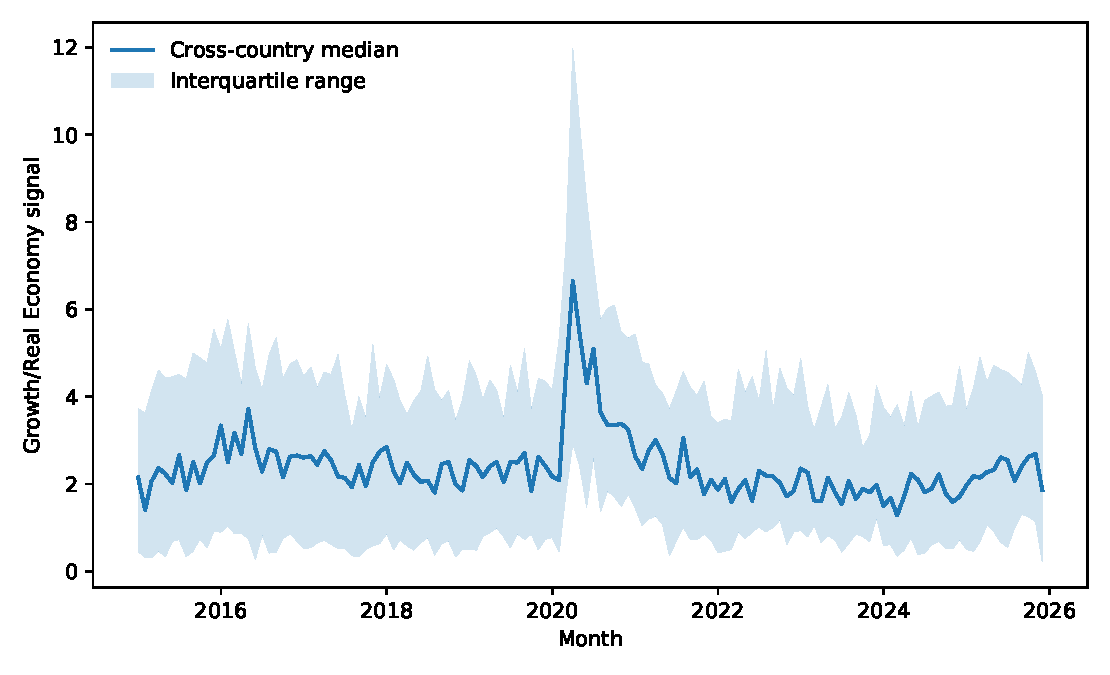
\includegraphics[width=0.82\textwidth]{Figure_0_GRE_Descriptive.pdf}
\caption{Cross-country distribution of the Growth/Real Economy news signal,
2015--2025. The line reports the monthly median and the shaded region the
interquartile range across available country observations.}
\label{fig:gre_descriptive}
\end{figure}

As a simple archive-depth check, we regress GRE on log retained article volume
over the 6,488 country-months with at least 100 articles. The coefficient is
0.103 with country fixed effects ($p=0.656$) and 0.100 with full month fixed
effects added ($p=0.713$). These do not establish representativeness, but they
give little evidence that GRE moves mechanically with article volume within
countries.

Let $x_i$ denote normalized headline and body text for article $i$. Economic
relevance is
\begin{equation}
R_i = \mathbf{1}\{x_i \text{ matches the economic-relevance dictionary}\}.
\label{eq:relevance}
\end{equation}
Articles that fail this screen receive zero risk score but stay in the
country-month denominator. This preserves the prevalence of economically
relevant reporting relative to the complete observed news flow.

The target-specific activation indicator is
\begin{equation}
G_i = \mathbf{1}\{x_i \text{ activates the Growth/Real Economy dictionary}\}.
\label{eq:growthdomain}
\end{equation}
The activation lexicon is small and fixed. In English it contains recession,
slowdown, contraction, unemployment, and layoffs, plus the corresponding French
and Portuguese terms used in production. Broader macro terms like GDP and
growth belong to the economic-relevance screen, not to GRE. That separation
keeps target-specific activation narrow and auditable; the full dictionaries
are in the replication package.\footnote{We fixed the GRE vocabulary before
forecasting. It was not selected by searching over term sets for the lowest
loss, which would be a form of specification search and would weaken the
predictive-accuracy tests.}

Relevant articles receive an ordinal severity score. Let $\mathcal{K}_i
\subseteq \{1,2,3,4\}$ be the severity tiers matched in article $i$:
\begin{equation}
S_i = \begin{cases}
0, & R_i = 0, \\
\max(\{1\} \cup \mathcal{K}_i), & R_i = 1.
\end{cases}
\label{eq:severity}
\end{equation}
Tier 1 is background or mild pressure; tier 2 is material deterioration; tier 3 is
severe disruption; tier 4 is extreme or systemic stress. The scale is ordinal and
not a recession probability.

Textual prominence uses a headline cue $T_i$, a body-length indicator $L_i$
for at least 1,200 normalized characters, and an indicator $M_i$ for
economically dense content activating at least two domains. The weight is
\begin{equation}
W_i = \operatorname{clip}(1 + 0.5 T_i + 0.2 L_i + 0.3 M_i, 1, 2),
\label{eq:weight}
\end{equation}
where $\operatorname{clip}(x,a,b)=\min\{\max(x,a),b\}$. These coefficients are
fixed. They are not estimated from GDP or tuned to minimize loss. Articles are
counted at most once per economic domain, so repeated keyword mentions do not
mechanically increase a domain's contribution. The robustness work keeps the
measurement rule fixed and tests exact-text duplication, article-volume
thresholds, signal transformations, tail caps, and theory-motivated
falsification domains. These checks test the corpus and signal choices, not the
dictionary, severity map, or emphasis weights.

The article contribution to GRE is
\begin{equation}
Q_i = R_i G_i S_i W_i.
\label{eq:article}
\end{equation}
A relevant article about a different domain has $G_i = 0$ and contributes
nothing to GRE. That is what separates GRE from broad AERI.

\begin{table}[htbp]
\centering\small
\caption{Construction of the Growth/Real Economy news signal}
\label{tab:construction}
\begin{tabularx}{\textwidth}{p{0.19\textwidth}X}
\toprule
Stage & Definition and interpretation \\
\midrule
Economic relevance $R_i$ & Indicator that normalized article text contains economically relevant content. Articles failing this screen contribute zero to the signal but remain in the country-month denominator. \\
Real-economy activation $G_i$ & Indicator that the article activates the frozen Growth/Real Economy dictionary: recession, slowdown, contraction, unemployment, layoffs, and the corresponding French and Portuguese activation terms. Broader GDP/growth vocabulary belongs to the economic-relevance screen rather than this target-specific activation rule. \\
Severity $S_i$ & Ordinal score for relevant articles: 1 = background or mild pressure; 2 = material deterioration; 3 = severe disruption; 4 = extreme or systemic real-economy stress. The highest matched tier applies. \\
Textual emphasis $W_i$ & $\operatorname{clip}(1+0.5T_i+0.2L_i+0.3M_i,1,2)$, where $T_i$ marks headline emphasis, $L_i$ marks at least 1,200 normalized characters, and $M_i$ marks economically dense multi-domain content. \\
Article contribution $Q_i$ & $Q_i=R_iG_iS_iW_i$. Only economically relevant articles that activate the real-economy domain contribute positive weight. \\
Country-month signal $GRE_{ct}$ & $100N_{ct}^{-1}\sum_{i\in\mathcal A_{ct}}Q_i$, where $N_{ct}$ is the total number of retained articles. The signal therefore reflects both the prevalence and the intensity of real-economy risk reporting. \\
\bottomrule
\end{tabularx}
\end{table}

\begin{table}[htbp]
\centering\scriptsize
\caption{Illustrative article-level mapping into the Growth/Real Economy signal}
\label{tab:worked_example}
\begin{tabularx}{\textwidth}{p{0.32\textwidth}cccccX}
\toprule
Stylized article content & $R_i$ & $G_i$ & $S_i$ & $W_i$ & $Q_i$ & Interpretation \\
\midrule
``Manufacturing output contracts sharply; factories announce layoffs and demand weakens'' & 1 & 1 & 3 & 2.0 & 6.0 & Economically relevant, activates the real-economy domain, severe language, and high textual emphasis. \\
``Foreign-exchange reserves decline while the currency comes under pressure'' & 1 & 0 & -- & -- & 0 & Economically relevant but does not activate the Growth/Real Economy domain, so it does not enter this signal. \\
Sports or entertainment article with no economic content & 0 & 0 & 0 & -- & 0 & Retained in the monthly article denominator but contributes zero to the numerator. \\
\bottomrule
\end{tabularx}
\vspace{0.3em}
\begin{minipage}{0.96\textwidth}\footnotesize\textit{Notes:} Examples are stylized illustrations, not quotations from the archive. For the first row, $W_i$ reaches its upper bound when all three emphasis indicators are active.\end{minipage}
\end{table}


For country $c$ and month $t$, let $\mathcal{A}_{ct}$ be the retained article
set and $N_{ct} = |\mathcal{A}_{ct}|$. The GRE signal is
\begin{equation}
GRE_{ct} = \frac{100}{N_{ct}} \sum_{i \in \mathcal{A}_{ct}} R_i G_i S_i W_i.
\label{eq:gre}
\end{equation}
The full article count stays in the denominator. GRE rises when real-economy
risk reporting becomes more prevalent, more severe, or more prominent. Define
\begin{equation}
B^G_{ct} = \frac{\sum_i R_i G_i}{N_{ct}}, \qquad
\overline{SW}^G_{ct} = \frac{\sum_i R_i G_i S_i W_i}{\sum_i R_i G_i}.
\label{eq:decomp_parts}
\end{equation}
Whenever the conditional denominator is positive,
\begin{equation}
GRE_{ct} = 100 \, B^G_{ct} \, \overline{SW}^G_{ct}.
\label{eq:decomp}
\end{equation}
This separates breadth of real-economy reporting from conditional severity and
prominence.

The closest construction-based comparator is broad AERI:
\begin{equation}
AERI_{ct} = \frac{100}{N_{ct}} \sum_{i \in \mathcal{A}_{ct}} R_i S_i W_i.
\label{eq:aeri_comp}
\end{equation}
The only difference is the absence of $G_i$. AERI asks whether general
economic-risk reporting is enough. GRE asks whether restricting the same
scored news flow to the real-economy domain gives a more useful variable. At
the forecasting stage we also report Inflation Risk and FX/External Risk as
economic falsification comparators. They do not enter GRE construction and
were not used to select or tune GRE.

\subsection{Annual GDP, temporal disaggregation, and information-set
admissibility}

The low-frequency panel covers all 54 African economies from 2015 to 2025. The
source workbook labels the annual series ``GDP (PPP)-WEO.'' The replication
package archives the exact workbook as supplied on 13 September 2026 and a
cleaned country-year extract. The workbook does not carry a WEO
publication-release identifier or vintage, so we do not infer one. We call
these annual observations ``final-vintage WEO-labelled benchmarks.''
``WEO-labelled'' refers to the label in the supplied workbook. It does not
identify an IMF WEO release, so no specific vintage is attributed.\footnote{The
phrase refers only to the label contained in the supplied workbook. Because
the workbook does not identify a specific IMF World Economic Outlook release,
no exact WEO vintage is inferred or attributed.}

Comparable official monthly GDP releases do not exist for the full African
panel. We build a monthly GDP-PPP activity proxy using additive first-difference
Denton disaggregation \citep{denton1971,imfqna2017}. For country $c$, let
$Y_{cy}$ be annual GDP-PPP and let $G^F_{ct}$ be the final-vintage monthly
proxy. The construction solves
\begin{equation}
\min_{\{G^F_{ct}\}} \sum_{t=2}^{T} \bigl(G^F_{ct} - G^F_{c,t-1}\bigr)^2
\quad \text{subject to} \quad
\sum_{m=1}^{12} G^F_{c,y,m} = Y_{cy} \;\; \forall y.
\label{eq:denton}
\end{equation}
The evaluation target is twelve-month growth:
\begin{equation}
y^F_{ct} = 100\bigl[\log G^F_{ct} - \log G^F_{c,t-12}\bigr].
\label{eq:gdp12}
\end{equation}
The superscript $F$ matters. This is an ex post final-vintage outcome proxy,
not a monthly series that anyone observed in real time.

For a fixed sample, Denton is a linear map from annual benchmarks to the
monthly vector. Write the annual vector as $Y^F$ and the monthly path as
\begin{equation}
G^F = H Y^F,
\label{eq:linear_operator}
\end{equation}
where $H$ is the matrix implied by the quadratic minimization and annual
aggregation constraints. At forecast origin $t$, split $Y^F = (Y^A_t, Y^U_t)$
into annual benchmarks that are available and unavailable under the historical
information rule, and split the columns of $H$ accordingly.

\paragraph{Information-set admissibility}
A constructed path is admissible at origin $t$ only if the rows used by the
model satisfy $H_{\leq t,U} = 0$, or if a one-sided reconstruction from
$Y^A_t$ is used instead. If $H_{\leq t,U} \neq 0$, then $G^F_{\leq t}$ depends
on annual information not available at $t$. A recursive forecast that uses
such values as lagged regressors, or admits targets before the annual
information needed to construct them has been released, is retrospective, not
pseudo-out-of-sample. The direction of the resulting distortion is ambiguous,
since both the benchmark and the estimated augmentation can change.

\paragraph{Proposition 1 (interior geometric decay of Denton benchmark
weights)}
Consider the additive first-difference Denton problem in
equation~\eqref{eq:denton} with $m=12$ months per annual block. Let
$t = (y_0, r)$ denote month $r \in \{1,\dots,12\}$ of year $y_0$, far enough
from the sample endpoints that the interior solution applies, and let $H_{t,y}$
be the weight of annual benchmark $Y_y$ in $G^F_t$. Under a constant annual
benchmark, the monthly solution is constant, so $\sum_y H_{t,y} = 1/12$. On
the doubly-infinite interior problem there exist month-specific constants
$C_r^{+}$ and $C_r^{-}$ such that, for every $k \geq 1$,
\begin{equation}
H_{t,y_0+k} = C_r^{+} \mu^{k-1}, \qquad
H_{t,y_0-k} = C_r^{-} \mu^{k-1},
\label{eq:denton_tail}
\end{equation}
where
\begin{equation}
\mu = \frac{12\sqrt{438}-289}{143} \approx -0.264745
\label{eq:denton_mu}
\end{equation}
is the unique stable root of
\begin{equation}
\frac{1}{3} + \frac{578}{429}z + \frac{1}{3}z^2 = 0.
\label{eq:denton_characteristic}
\end{equation}
Hence $|H_{t,y_0 \pm k}| = O(|\mu|^k)$, and, once the off-diagonal tail is
entered, each additional annual step multiplies its magnitude by
$|\mu| \simeq 0.2647$ and reverses its sign. The first unavailable-year
coefficient is not a fixed fraction of the own-year coefficient: its level and
sign depend on the month $r$. The geometric rate governs the subsequent tail
exactly in the interior limit.

\paragraph{Derivation}
Let $e_y = G^F_{12y}$ be the year-end monthly level. Conditional on adjacent
endpoints, the twelve within-year first differences solve a two-constraint
minimum-norm problem. Eliminating those local differences gives a quadratic
criterion in $(e_{y-1}, e_y, Y_y)$. The interior first-order condition for the
shared boundary $e_y$ is
\begin{equation}
\frac{1}{3} e_{y-1} + \frac{578}{429} e_y + \frac{1}{3} e_{y+1}
= \frac{Y_y}{11} + \frac{Y_{y+1}}{13}.
\label{eq:denton_boundary_recursion}
\end{equation}
Away from the two annual blocks directly forced by a given benchmark, the
response obeys the homogeneous second-order recurrence associated with
equation~\eqref{eq:denton_characteristic}. Its roots are reciprocal;
boundedness selects $\mu$, which gives equation~\eqref{eq:denton_tail}.
Back-substitution into the local twelve-month solution produces the exact
month-specific coefficients. The full Schur-complement derivation, the
within-year weight profile, and a finite-sample cross-check for the 2015--2025
construction are in the online supplement. This geometric impulse-response
structure is characteristic of banded difference-penalty smoothers; the point
here is to use it to quantify forecast-origin information leakage, not to
introduce a new smoothing method \citep{eilers2003}.

Two implications follow. Leakage is concentrated in nearby annual blocks:
after the first off-diagonal coefficient, one more year retains about 26.5
percent of its magnitude, two more years about 7.0 percent, four more years
under 0.5 percent. And because $\mu < 0$, successive annual contributions
alternate in sign. Denton look-ahead therefore has no favourable direction:
depending on month, horizon, and benchmark, it can raise or lower relative
loss. The rapid decay is also why the May, July, and November release
conventions differ mainly in how they treat the nearest unavailable benchmark,
not in a long tail of distant years.

The admissibility condition extends \citet{croushorestark2001} to constructed
targets. It does not say temporal disaggregation is wrong. What matters is the
role the disaggregated path plays in the forecast experiment. A final-vintage
path can be a legitimate outcome and still be inadmissible as forecast-origin
information.

Figure~\ref{fig:leakage} summarizes the distinction. The upper path is valid
for retrospective description and ex post scoring but becomes inadmissible if
the full constructed history is fed into a historical forecast origin. The
lower path separates origin-available GDP information from the final-vintage
outcome observed later for evaluation.

\begin{figure}[htbp]
\centering
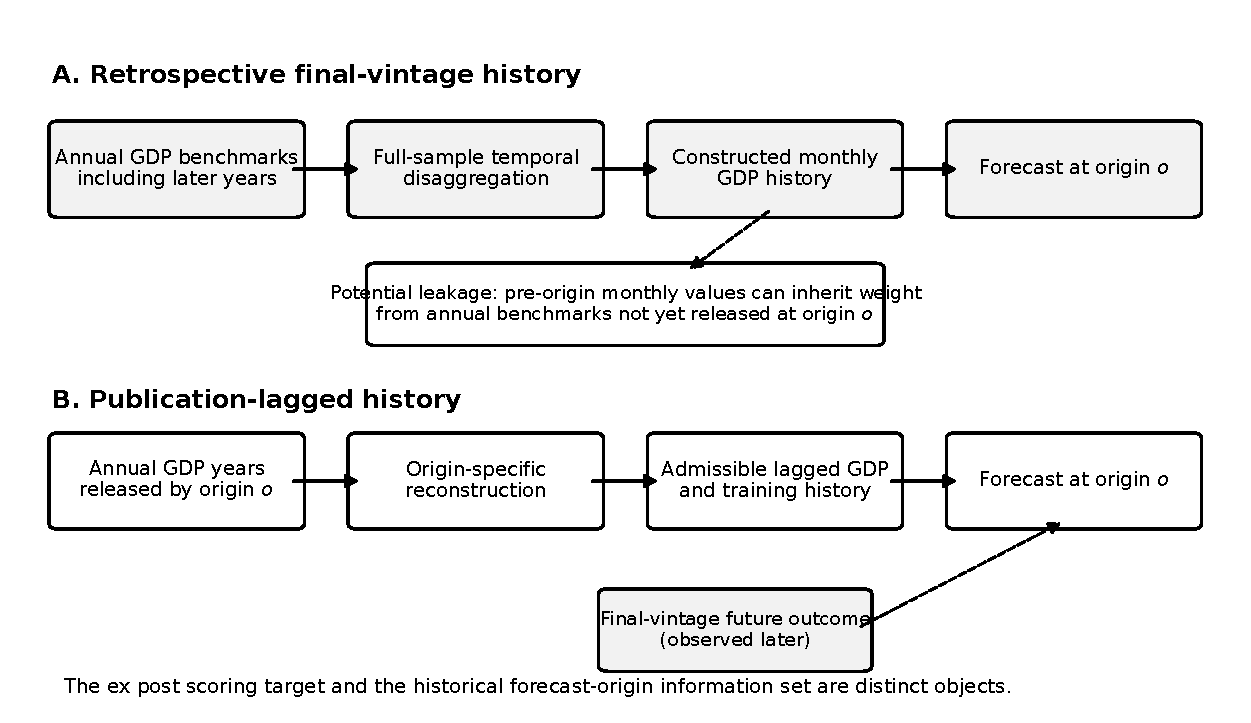
\includegraphics[width=0.96\textwidth]{Figure_Target_Information_Leakage.pdf}
\caption{Target-information leakage in retrospective versus publication-lagged
forecast construction.}
\label{fig:leakage}
\begin{singlespace}\footnotesize\textit{Notes:} The retrospective path may
allow unreleased annual benchmarks to influence pre-origin monthly values
through temporal disaggregation. The publication-lagged path reconstructs
lagged GDP and training information using only annual years permitted at the
forecast origin. A final-vintage future outcome can still be used later for
scoring without being treated as information available at the origin.
\end{singlespace}
\end{figure}

\subsection{Publication-lagged reconstruction}

Using $G^F_{ct}$ directly as a lagged predictor would let future annual
benchmarks shape the historical monthly path. We reconstruct the GDP
information set separately at every forecast origin $s$. Under the baseline
release rule, the latest annual benchmark year permitted at origin $s$ is
\begin{equation}
a(s) = \begin{cases}
\operatorname{year}(s) - 1, & \operatorname{month}(s) \geq 5, \\
\operatorname{year}(s) - 2, & \operatorname{month}(s) < 5.
\end{cases}
\label{eq:availyear}
\end{equation}
Only annual benchmarks through $a(s)$ enter the Denton problem. For months
after December of $a(s)$ and up to the forecast origin, the monthly path is
extrapolated using the constant log-monthly rate implied by the two most
recent permitted annual totals,
\begin{equation}
r_{c,s} = \frac{1}{12}\bigl[\log Y_{c,a(s)} - \log Y_{c,a(s)-1}\bigr],
\label{eq:extraprate}
\end{equation}
with a zero trend if only one annual benchmark is available. This gives an
origin-specific path $G^{I(s)}_{ct}$ and corresponding lagged twelve-month
growth $y^{I(s)}_{ct}$. The same release rule governs recursive training: an
outcome dated in calendar year $y$ is eligible for estimation only from May of
$y+1$. We repeat the exercise with July and November release
months.\footnote{The May rule is an operational convention, not a claim that
all 54 economies publish annual GDP on a common date. The July and November
exercises show whether the conclusions depend on a relatively early
annual-information assumption.}

The rule is transparent but does not solve revision uncertainty. Annual
observations through $a(s)$ are still taken from the final-vintage file, not
from archived contemporaneous releases. The design therefore prevents
mechanical use of future years but does not remove information embedded in
later revisions to already released years. We say ``publication-lagged
final-vintage,'' not ``real-time.''

\section{Forecast design and simulation evidence}

\subsection{Publication-lagged forecast design and inference}

Country membership and text scaling are fixed before evaluation. GRE and
comparators are standardized within country on 2015--2018, frozen before
January 2020. No country was selected on the basis of a news--GDP correlation,
coefficient sign, or evaluation-period forecast performance.

For horizon $h$, the benchmark is
\begin{equation}
y^F_{c,t+h} = \alpha_c + \sum_{j=0}^{2}\phi_{j,h} y^{I(t)}_{c,t-j}
+ \sum_{m=2}^{12}\delta_{m,h}\mathbf{1}\{M_{t+h}=m\} + u_{c,t+h},
\label{eq:benchmark}
\end{equation}
where the three GDP-growth lags come from the information set available at
origin $t$. The GRE specification adds standardized GRE measured at $t$.
Parameters are re-estimated recursively over expanding samples subject to the
target-release rule. Target dates span January 2020--December 2025, and
forecast horizons are 1, 3, 6, and 12 months. The target-timing correction was
introduced after the earlier 12-month specification had been examined. We
therefore report the full horizon profile and do not relabel the one-month
horizon as pre-specified.

\begin{table}[htbp]
\centering\scriptsize\singlespacing
\caption{Publication-lagged final-vintage forecasting design}
\label{tab:design}
\renewcommand{\arraystretch}{0.92}
\begin{tabularx}{\textwidth}{p{0.24\textwidth}X}
\toprule
Element & Implementation \\
\midrule
Country universe & Fifty-four African economies; membership is determined by pre-evaluation data availability only. \\
Annual GDP source & Author-supplied annual series labelled ``GDP (PPP)-WEO,'' 2015--2025. The replication copy is frozen as supplied on 13 September 2026. The workbook does not identify the underlying WEO publication vintage, so the annual values are treated as final-vintage data rather than historical real-time vintages. \\
Realized evaluation target & Twelve-month growth of a final-vintage monthly GDP-PPP proxy constructed by additive first-difference Denton and constrained to aggregate exactly to the annual benchmarks. This series is used only to score realized forecast outcomes. \\
Forecast-origin GDP information & At each forecast origin, lagged monthly GDP growth is reconstructed from annual benchmark years permitted by the release rule. Under the baseline rule, year $y$ becomes usable from May of $y+1$. Denton is applied only through the last permitted annual year; subsequent months up to the forecast origin are extrapolated using the log-monthly rate implied by the two most recent permitted annual totals. \\
Training-target availability & A realized target dated in calendar year $y$ enters recursive estimation only from May of $y+1$ under the baseline rule. \\
Text scaling & Country-specific GRE and comparator means and standard deviations are estimated over 2015--2018 and frozen before the January 2020 evaluation start. \\
Benchmark & Pooled country-fixed-effects autoregression using three publication-lagged GDP-growth lags and target-month seasonal indicators. GRE adds one standardized news regressor at the forecast origin. \\
Evaluation & Recursive target dates January 2020--December 2025 at 1-, 3-, 6-, and 12-month forecast horizons. The full horizon profile is reported; no new horizon is relabelled as pre-specified after inspection of the corrected results. \\
Release-timing sensitivity & Baseline May availability is repeated using July and November release conventions. \\
Inference & RMSFE, MAE, target-month HAC Clark--West inference, complementary two-way country--target-month covariance, Holm correction across horizons, cross-section-preserving moving-block bootstrap, and country-level RMSFE ratios. \\
\bottomrule
\end{tabularx}
\end{table}


Forecast accuracy is summarized by RMSFE and MAE. Nested comparisons use the
Clark--West adjusted loss differential \citep{clarkwest2007}.\footnote{For
nested models, estimating an additional coefficient can raise the augmented
model's raw mean-squared forecast error even when the added predictor contains
useful population information. The Clark--West adjustment corrects for this
estimation-noise effect. Raw-loss and adjusted-loss tests therefore answer
related but distinct questions, which is why we report both.} Our main
dependence-robust calculation averages the Clark--West differential across
countries within a target month and applies Newey--West HAC inference with
horizon-appropriate overlap lags. This keeps the contemporaneous cross-section
rather than treating country errors as independent. As a diagnostic we also
report observation-level two-way covariance clustered by country and target
month, motivated by the panel forecast-comparison literature
\citep{qu2024,akgun2024,coroneo2025}. We apply Holm correction across the four
horizons and use a moving-block bootstrap that resamples 12-month target-date
blocks while preserving all countries within each selected
month.\footnote{Resampling target dates rather than individual country
observations preserves the contemporaneous cross-country dependence in the
forecast-error panel. The 12-month block length accommodates the overlap
induced by the twelve-month growth target.}

Cross-sectional dependence remains substantial after the information
correction. For the one-month benchmark, the balanced diagnostic panel has 53
countries over 72 target months, the mean pairwise forecast-error correlation
is about 0.442, and the Pesaran CD statistic is about 139.2. Dependence-aware
inference is therefore necessary.

\subsection{Monte Carlo design}

A single application cannot show how information timing behaves across
different DGPs. We therefore use two Monte Carlo designs to isolate the
information-set channel. Each replication has 54 economies and a monthly
calendar from 2015 through 2025. Annual GDP follows a panel process with
country-specific average growth, a common annual component, and idiosyncratic
innovations. Annual flows are converted to monthly frequency with the same
first-difference Denton operator used in the application. Forecasts condition
on three lags of twelve-month growth and country fixed effects. To isolate
target-information treatment, the simulations use a fixed pre-evaluation
estimation window and evaluate 2020--2025.

The first DGP is modest by design. The alternative-data variable measures the
contemporaneous annual activity innovation with noise and contains no
next-year innovation. Its scale is set so that, under feasible publication
timing, the one-month improvement is small and of the same order as the
corrected empirical result. The second design is a persistent-state stress DGP.
It raises annual persistence and the signal-to-noise ratio specifically to test
whether retrospective final-vintage information can produce the direction of
the empirical 12-month reversal. Its parameters are chosen for this stress
exercise rather than to fit the African data or reproduce the complete
empirical horizon profile. A separate placebo replaces the signal with
independent noise.

For every DGP we compare two information treatments. The retrospective design
supplies the complete final-vintage Denton history to the model. The
publication-lagged design admits annual benchmark $y$ only from May of $y+1$
and extrapolates between releases, exactly as in the empirical baseline. We
report 1,000 replications for each signal design and keep the pure-noise
placebo as a falsification check.

\subsection{Monte Carlo results}

\begin{table}[htbp]
\centering
\small
\caption{Monte Carlo: target-information treatment and the horizon profile of text value}
\label{tab:simulation}
\resizebox{\textwidth}{!}{%
\begin{tabular}{@{}llrrr@{}}
\toprule
DGP & Design & $h$ & Mean relative RMSFE & Share with RMSFE gain \\
\midrule
Current-state signal & Retrospective final-vintage & 1 & 1.0002 & 39.0\% \\
Current-state signal & Publication-lagged & 1 & 0.9969 & 97.7\% \\
Current-state signal & Retrospective final-vintage & 3 & 1.0002 & 36.6\% \\
Current-state signal & Publication-lagged & 3 & 0.9973 & 96.5\% \\
Current-state signal & Retrospective final-vintage & 6 & 1.0002 & 39.2\% \\
Current-state signal & Publication-lagged & 6 & 0.9987 & 84.6\% \\
Current-state signal & Retrospective final-vintage & 12 & 1.0001 & 47.5\% \\
Current-state signal & Publication-lagged & 12 & 1.0025 & 47.6\% \\
\midrule
Persistent-state stress & Retrospective final-vintage & 12 & 0.9962 & 90.2\% \\
Persistent-state stress & Publication-lagged & 12 & 1.0122 & 35.1\% \\
\bottomrule
\end{tabular}}
\begin{singlespace}\footnotesize\textit{Notes:} 1,000 replications per DGP with 54 economies and a 2015--2025 monthly calendar. The current-state signal is calibrated to a modest feasible short-horizon effect and contains no next-year innovation. The persistent-state stress DGP deliberately increases persistence and signal-to-noise to test whether retrospective final-vintage information can reproduce the direction of the empirical 12-month reversal; it is an existence calibration, not an empirical mechanism estimate. A separate pure-noise placebo remains approximately neutral under both information treatments. Full horizon results for all three DGPs appear in the online supplement.\end{singlespace}
\end{table}


\begin{figure}[htbp]
\centering
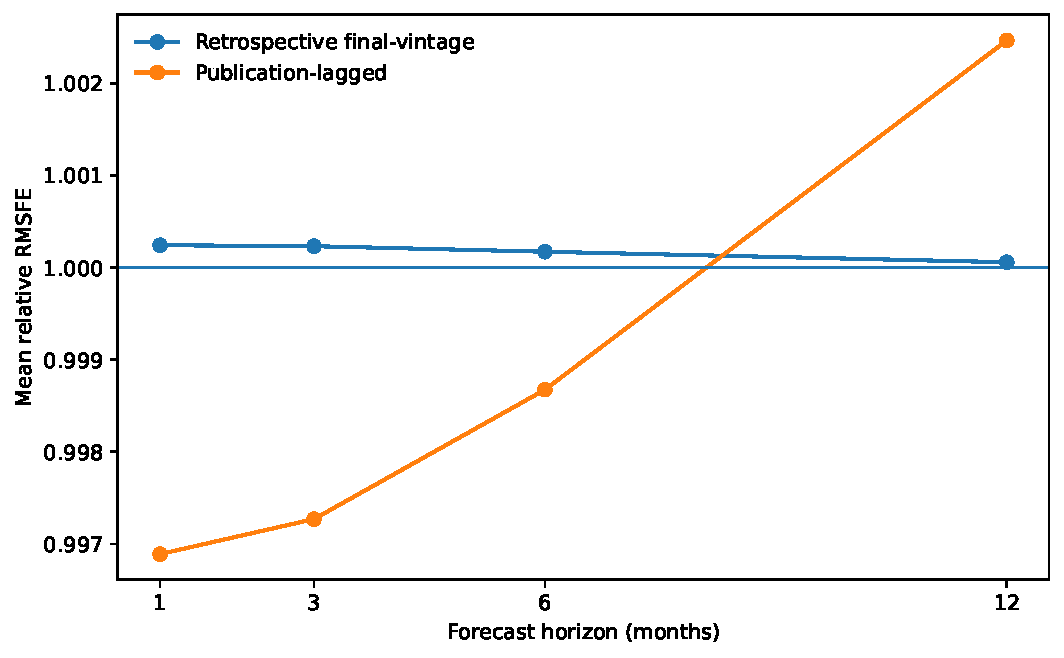
\includegraphics[width=0.76\textwidth]{Figure_Simulation_Horizon_Distortion.pdf}
\caption{Baseline Monte Carlo horizon profile under retrospective and
publication-lagged target information.}
\label{fig:simulation}
\begin{singlespace}\footnotesize\textit{Notes:} Lines report mean relative
RMSFE across 1,000 replications for the modest current-state-signal DGP. Values
below one favour the text-augmented model. The persistent-state stress
calibration is summarized in Table~\ref{tab:simulation} and reported fully in
the online supplement.\end{singlespace}
\end{figure}

The two DGPs show different distortions. In the modest current-state design,
publication-lagged information reveals short-horizon value that the
retrospective specification almost completely suppresses. Mean one-month
relative RMSFE is 0.9969 under publication-lagged information but 1.0002 under
retrospective final-vintage information. At twelve months, the retrospective
ratio is 1.0001 and the publication-lagged ratio is 1.0025. Information-set
treatment therefore changes the magnitude and horizon profile of the signal,
while the long-horizon comparison in this design remains near one rather than
matching the empirical reversal.

The persistent-state calibration produces the long-horizon reversal. With
high annual persistence and a stronger signal, mean 12-month relative RMSFE is
0.9962 under retrospective final-vintage information and 1.0122 under
publication-lagged information. The direction matches the African reversal,
where 0.9961 becomes 1.0048. Because the stress DGP generates much larger
short-horizon effects than the data, it is an existence result rather than a
calibrated account of the African pattern. It shows that, under plausible
persistence and signal-to-noise, an admissibility violation can create an
apparent long-horizon advantage that disappears once the information set is
made feasible.\footnote{The stress parameters are set to generate the direction
of the empirical-style reversal rather than estimated from the African panel.
The simulation establishes the possibility of this distortion without
identifying the mechanism behind the observed African reversal.}

Across the two designs, final-vintage target information masks a short-horizon
signal in one DGP and creates an apparent long-horizon gain in another. The
pure-noise placebo remains near neutral. The sign of the distortion is therefore
unrestricted and depends on the persistence and signal structure of the DGP.

\section{Empirical application: African GDP forecasting}

\subsection{Target-information audit}

Table~\ref{tab:target_audit} makes the look-ahead issue concrete. The earlier
design used the final-vintage Denton series both as the realized target and as
lagged GDP information. That gave a 12-month relative RMSFE of 0.9961 with
nominal Clark--West $p = 0.033$. Once forecast-origin GDP lags are
reconstructed from publication-permitted years and training outcomes are
delayed to their assumed release date, the 12-month relative RMSFE becomes
1.0048. The long-horizon advantage disappears. What remains is at one and
three months.

\begin{table}[htbp]
\centering\small\singlespacing
\caption{Target-information audit: final-vintage lags versus publication-lagged lags}
\label{tab:target_audit}
\begin{tabularx}{\textwidth}{p{0.35\textwidth}rrX}
\toprule
Design & Horizon & Relative RMSFE & Interpretation \\
\midrule
Final-vintage monthly GDP treated as available at origin & 12 & 0.9961 & Retrospective diagnostic only; nominal CW $p=0.033$. \\
Publication-lagged GDP information set & 12 & 1.0048 & No long-horizon GRE gain; HAC CW $p=0.905$. \\
Publication-lagged GDP information set & 1 & 0.9964 & Modest short-horizon predictive content; HAC CW $p=0.0006$. \\
\bottomrule
\end{tabularx}
\vspace{0.35em}
\begin{minipage}{0.97\textwidth}\footnotesize\textit{Notes:} The first row reproduces the earlier working specification in which the final-vintage temporally disaggregated GDP proxy was also used as forecast-origin lag information. Because that monthly path incorporates annual benchmarks not available at historical origins, it is not used as pseudo-out-of-sample evidence in the revised paper. The corrected design uses the final-vintage series only as the realized outcome and reconstructs forecast-origin GDP information under explicit release lags.\end{minipage}
\end{table}


\subsubsection{Formal design-difference test and channel decomposition}

The audit changes two things at once: the lagged GDP history observed at the
origin, and the date when realized target observations enter recursive
estimation. To separate them, define four nested designs. $R$ is the original
retrospective design with final-vintage GDP lags and immediate training; $L$
corrects only the forecast-origin GDP lags; $T$ corrects only training-outcome
availability; and $P$ applies both. Let $\rho_d$ be GRE RMSFE divided by
benchmark RMSFE under design $d \in \{R,L,T,P\}$. The total design effect is
\[
\Delta_{P-R} = \rho_P - \rho_R.
\]
Since the two corrections interact, we allocate their contributions
symmetrically with a two-factor Shapley decomposition,
\[
\phi_{\mathrm{lag}} = \tfrac12\bigl[(\rho_L - \rho_R) + (\rho_P - \rho_T)\bigr],
\qquad
\phi_{\mathrm{train}} = \tfrac12\bigl[(\rho_T - \rho_R) + (\rho_P - \rho_L)\bigr],
\]
so that $\phi_{\mathrm{lag}} + \phi_{\mathrm{train}} = \Delta_{P-R}$ exactly.
Inference for these nonlinear RMSFE-ratio contrasts uses 5,000 circular
moving-block draws of 12 consecutive target months, keeping all countries in
each resampled month.

\begin{table}[htbp]
\centering\small
\caption{Formal decomposition of the 12-month target-information correction}
\label{tab:channel_decomposition}
\begin{tabularx}{\textwidth}{@{}>{\raggedright\arraybackslash}Xcc@{}}
\toprule
\multicolumn{3}{l}{\textit{Panel A. Nested information-set designs}} \\
Design & Relative RMSFE & Relative MAE \\
\midrule
Retrospective: final-vintage lags + immediate training & 0.9961 & 0.9930 \\
GDP-lag corrected only & 1.0017 & 1.0070 \\
Training-timing corrected only & 0.9966 & 0.9967 \\
Fully publication-lagged & 1.0048 & 1.0122 \\
\midrule
\multicolumn{3}{l}{\textit{Panel B. Paired 12-month block-bootstrap decomposition of relative RMSFE}} \\
Contrast & Change in relative RMSFE & 95\% bootstrap interval \\
\midrule
Total correction, $P-R$ & +0.0088 & [+0.0048, +0.0171] \\
GDP-lag channel, Shapley contribution & +0.0069 & [+0.0042, +0.0145] \\
Training-timing channel, Shapley contribution & +0.0018 & [-0.0018, +0.0075] \\
\bottomrule
\end{tabularx}
\begin{minipage}{0.97\textwidth}\footnotesize\textit{Notes:} $R$ uses final-vintage GDP lags and immediate inclusion of realized training outcomes; $L$ corrects only the forecast-origin GDP lags; $T$ corrects only training-outcome availability; and $P$ applies both corrections. Panel B reports the nonlinear difference in relative RMSFE and a two-channel Shapley decomposition, so the two channel contributions sum exactly to the total $P-R$ change. The 5,000-draw circular moving-block bootstrap resamples 12-month target-date blocks and preserves the full contemporaneous cross-section. The total and GDP-lag intervals exclude zero; the training-timing interval includes zero. Complementary direct tests on country-month loss-gain differences are reported in the text and replication files.\end{minipage}
\end{table}


At twelve months, relative RMSFE moves from 0.9961 under $R$ to 1.0017 when
only the GDP-lag history is corrected, 0.9966 when only training timing is
corrected, and 1.0048 under the full correction $P$. The total $P-R$ change is
$+0.0088$, with a paired block-bootstrap 95 percent interval of
$[0.0048, 0.0171]$. The Shapley contribution of the GDP-lag channel is
$+0.0069$ ($[0.0042, 0.0145]$), about 79 percent of the total. The
training-timing contribution is $+0.0018$, and its interval
$[-0.0018, 0.0075]$ includes zero. The reversal is therefore mainly about
replacing the retrospective GDP history, not about when realized outcomes
enter recursive training.

Complementary tests on country-month loss-gain differences are more
conservative. For the total 12-month correction, the two-sided raw-loss
contrast gives target-month HAC $p = 0.100$ and two-way $p = 0.137$, while the
Clark--West-gain contrast gives $p = 0.148$ and $p = 0.159$. The GDP-lag
component of the raw-loss change is significant at conventional levels (HAC
$p = 0.020$; two-way $p = 0.049$), with the Clark--West version marginal
(0.054 and 0.074). Reporting both forms of inference matters: the paired
bootstrap tests the reported relative-RMSFE change directly, whereas
observation-level adjusted-loss contrasts are less precise about the total
design difference.\footnote{The two inferential objects are not algebraically
equivalent, because each information design changes the benchmark forecast and
so the denominator of relative RMSFE. The paired block bootstrap evaluates the
reported relative-RMSFE contrast directly; the HAC and two-way calculations
instead test changes in raw or Clark--West-adjusted country-month loss gains.}

The reversal has a clear implication: a constructed high-frequency target
cannot serve at once as an ex post outcome and as if its final-vintage history
had been observable to the forecaster. The retrospective final-vintage
result is kept in the replication package only as an audit trail; it is not
used to support the predictive claim.

Figure~\ref{fig:empirical_reversal} shows the full horizon profile under both
information treatments. The correction is not a small adjustment to inference:
it changes where the apparent advantage occurs and reverses the sign of the
12-month comparison.

\begin{figure}[htbp]
\centering
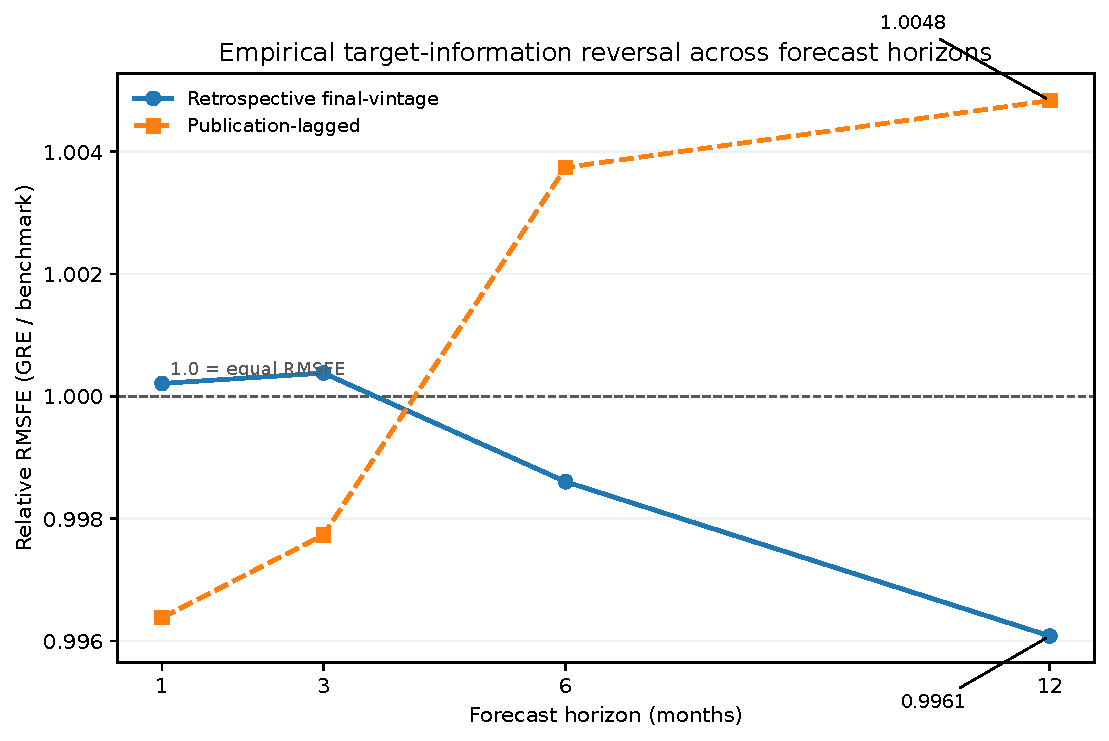
\includegraphics[width=0.82\textwidth]{Figure_Empirical_Horizon_Reversal.pdf}
\caption{Empirical horizon profile under retrospective final-vintage and
publication-lagged information.}
\label{fig:empirical_reversal}
\begin{singlespace}\footnotesize\textit{Notes:} Relative RMSFE below one
favours GRE. The retrospective specification uses the full final-vintage
Denton history as lagged GDP information. The publication-lagged specification
reconstructs forecast-origin GDP histories using only annual benchmark years
permitted by the release rule.\end{singlespace}
\end{figure}

\subsection{Corrected horizon profile and release timing}

Table~\ref{tab:main_results} reports the publication-lagged comparison. The
correction changes the horizon profile, not just the standard errors. At one
month, benchmark RMSFE is 8.375 and GRE RMSFE is 8.344, for a ratio of 0.9964.
MAE falls from 5.441 to 5.385, giving relative MAE 0.9897. At three months,
relative RMSFE is 0.9977 and relative MAE is 0.9928. At six and twelve months
the RMSFE ratios rise above one, to 1.0037 and 1.0048.

\begin{table}[htbp]
\centering\scriptsize
\caption{Publication-lagged forecast performance of the GRE-augmented model}
\label{tab:main_results}
\resizebox{\textwidth}{!}{%
\begin{tabular}{rrrrrrrr}
\toprule
$h$ & Benchmark RMSFE & GRE RMSFE & Rel. RMSFE & Benchmark MAE & GRE MAE & HAC CW $p$ & Two-way $p$ \\
\midrule
1  & 8.375 & 8.344 & 0.9964 & 5.441 & 5.385 & 0.0006 & 0.053 \\
3  & 8.493 & 8.473 & 0.9977 & 5.523 & 5.483 & 0.041 & 0.084 \\
6  & 8.588 & 8.620 & 1.0037 & 5.513 & 5.529 & 0.878 & 0.869 \\
12 & 19.264 & 19.357 & 1.0048 & 7.028 & 7.114 & 0.905 & 0.872 \\
\bottomrule
\end{tabular}}
\vspace{0.35em}
\begin{minipage}{0.97\textwidth}\footnotesize\textit{Notes:} The dependent variable is final-vintage twelve-month GDP-PPP proxy growth. Forecast-origin GDP lags and the recursive training sample obey the baseline May release rule described in Table~\ref{tab:design}. Relative RMSFE below one indicates lower forecast loss. Holm adjustment across the four target-month HAC tests gives adjusted $p=0.0023$ at $h=1$ and $p=0.122$ at $h=3$. The corresponding two-way adjusted values are 0.211 and 0.253.\end{minipage}
\end{table}


At one month, target-month HAC Clark--West inference gives $p = 0.0006$. The
complementary two-way country--target-month value is $p = 0.053$. Holm
correction across the four HAC horizon tests gives adjusted $p = 0.0023$ at one
month and 0.122 at three months; the two-way adjusted values are larger. A
5,000-draw target-month moving-block bootstrap gives a one-sided Clark--West
value of $p = 0.037$. The raw percentage RMSFE improvement is about 0.36
percent, and its 95 percent bootstrap interval is approximately
$[-0.50, 1.44]$, so the magnitude remains imprecisely estimated even though the
adjusted-loss evidence is favourable. Country-level RMSFE is lower with GRE in
33 of 54 economies, with a median country ratio of about 0.991.

The corrected evidence is therefore modest. It suggests some incremental
information in GRE for the next few observations of twelve-month GDP growth
when the conventional GDP information set is publication constrained.

\subsubsection{Excluding 2020--2021}

Pandemic-era observations are unusually volatile in both macroeconomic
outcomes and news intensity, so the main result could reflect the 2020--2021
episode rather than the target-information problem. We therefore repeat the
full horizon exercise using only January 2022--December 2025 as forecast
targets, keeping the same pre-evaluation history, recursive estimation rules,
and information-set conventions.

\begin{table}[htbp]
\centering
\caption{Forecast robustness excluding the 2020--2021 pandemic period}
\label{tab:excovid}
\begin{tabular}{llcccc}
\toprule
Sample & Information design & $h=1$ & $h=3$ & $h=6$ & $h=12$ \\
\midrule
2020--2025 & Retrospective & 1.0002 & 1.0004 & 0.9986 & 0.9961 \\
2020--2025 & Publication-lagged & 0.9964 & 0.9977 & 1.0037 & 1.0048 \\
2022--2025 & Retrospective & 1.0001 & 1.0002 & 0.9995 & 0.9976 \\
2022--2025 & Publication-lagged & 0.9926 & 0.9929 & 0.9988 & 1.0133 \\
\midrule
\multicolumn{6}{l}{\textit{Publication-lagged 2022--2025 inference}} \\
Horizon & Relative MAE & \multicolumn{2}{c}{CW HAC $p$} & \multicolumn{2}{c}{CW two-way $p$} \\
\midrule
1 month & 0.9863 & \multicolumn{2}{c}{$<0.001$} & \multicolumn{2}{c}{0.0271} \\
3 months & 0.9887 & \multicolumn{2}{c}{0.0014} & \multicolumn{2}{c}{0.0289} \\
6 months & 0.9978 & \multicolumn{2}{c}{0.0811} & \multicolumn{2}{c}{0.1583} \\
12 months & 1.0229 & \multicolumn{2}{c}{0.9697} & \multicolumn{2}{c}{0.7706} \\
\bottomrule
\end{tabular}
\begin{minipage}{0.97\textwidth}\footnotesize\textit{Notes:} Entries in the first panel are GRE RMSFE divided by the corresponding benchmark RMSFE. The restricted evaluation sample begins in January 2022 and ends in December 2025, removing all 2020--2021 forecast targets while retaining the same recursive estimation history and information-set rules. The publication-lagged 12-month ratio remains above one after the exclusion, whereas the retrospective ratio remains below one. The one- and three-month publication-lagged comparisons strengthen in the restricted sample. Clark--West values are one-sided tests of incremental predictive content, with target-month HAC and complementary country$\times$target-month two-way covariance.\end{minipage}
\end{table}


The reversal becomes more pronounced outside the pandemic. At twelve months,
the retrospective specification still suggests a small GRE gain, with relative
RMSFE 0.9976, while the publication-lagged ratio rises to 1.0133. At one
month, by contrast, the corrected GRE comparison strengthens from 0.9964 in
the full sample to 0.9926 after 2020--2021 is removed; relative MAE is 0.9863,
target-month HAC Clark--West $p < 0.001$, and the complementary two-way value
is $p = 0.027$. The three-month ratio is 0.9929 with HAC $p = 0.0014$ and
two-way $p = 0.029$, whereas six months is near neutral and twelve months is
unfavourable. The information-set reversal does not come from the
extraordinary 2020--2021 observations. If anything, the non-pandemic sample
sharpens the distinction between short-horizon GRE information and the absence
of a robust long-horizon advantage.

The baseline May rule is an availability convention, not an exact release date
for every African economy. Table~\ref{tab:release_timing} therefore repeats the
whole origin-specific reconstruction using July and November of the following
year. The one-month GRE result remains favourable under both more conservative
rules. Relative RMSFE is 0.9969 under July availability and 0.9973 under
November availability; relative MAE stays near 0.99. Target-month HAC values
remain below 0.001, two-way values are 0.039 and 0.030, and bootstrap
Clark--West values are 0.038 and 0.019. Between 31 and 33 of 54 countries have
lower one-month RMSFE across the three conventions.

\begin{table}[htbp]
\centering\small
\caption{Sensitivity of the one-month GRE result to annual-data release timing}
\label{tab:release_timing}
\resizebox{\textwidth}{!}{%
\begin{tabular}{lrrrrrr}
\toprule
Annual year $y$ usable from & Rel. RMSFE & Rel. MAE & HAC CW $p$ & Two-way $p$ & Bootstrap CW $p$ & Countries $<1$ \\
\midrule
May of $y+1$ & 0.9964 & 0.9897 & 0.0006 & 0.053 & 0.037 & 33/54 \\
July of $y+1$ & 0.9969 & 0.9894 & 0.0004 & 0.039 & 0.038 & 31/54 \\
November of $y+1$ & 0.9973 & 0.9910 & 0.0001 & 0.030 & 0.019 & 32/54 \\
\bottomrule
\end{tabular}}
\vspace{0.35em}
\begin{minipage}{0.97\textwidth}\footnotesize\textit{Notes:} Each row reconstructs the GDP information set and recursive training eligibility under the stated release convention. Bootstrap results use 5,000 moving-block replications with 12-month target-date blocks and preserve the contemporaneous country cross-section.\end{minipage}
\end{table}


This robustness matters because we do not have archived release dates or
historical annual vintages for every country. The result is not tied to
treating annual data as available immediately after year-end.

\subsection{Loss uncertainty, country breadth, and domain alignment}

At the one-month horizon, 82.6 percent of 5,000 moving-block replications imply
a lower raw RMSFE under GRE. The 95 percent interval for the percentage RMSFE
improvement is about $[-0.50, 1.44]$, while the bootstrap Clark--West one-sided
value is 0.037. We report the difference between raw-loss uncertainty and
nested-model adjusted-loss inference directly rather than resolving it by
choosing one statistic. Country-level evidence is heterogeneous: 33 of 54
economies have lower RMSFE and 21 do not, though the median country ratio is
about 0.991.

Figure~\ref{fig:country_heterogeneity} reports all country-level ratios rather
than reducing the heterogeneity to a single count. The dispersion reinforces
that the pooled result is an average short-horizon signal, not uniform
country-level dominance.

\begin{figure}[p]
\centering
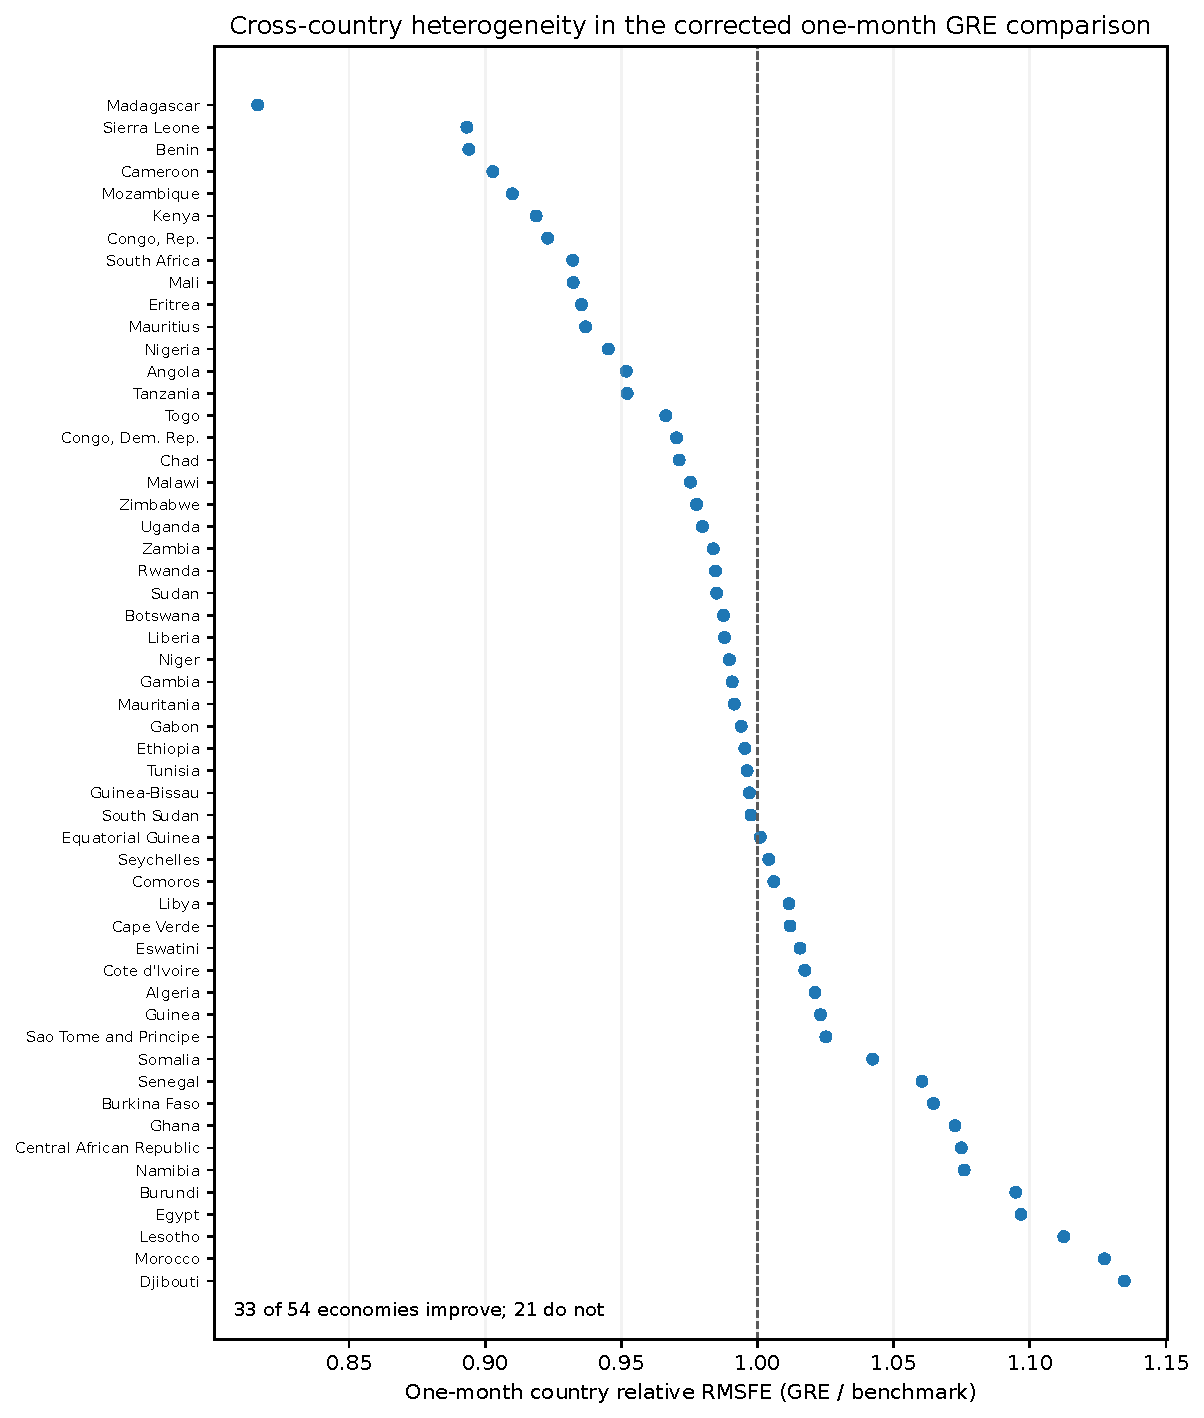
\includegraphics[width=0.88\textwidth,height=0.84\textheight,keepaspectratio]{Figure_Country_Heterogeneity.pdf}
\caption{Cross-country heterogeneity in the corrected one-month GRE
comparison.}
\label{fig:country_heterogeneity}
\begin{singlespace}\footnotesize\textit{Notes:} Each point is a country's
one-month RMSFE from the GRE-augmented model divided by the corresponding
publication-lagged benchmark RMSFE. Values below one indicate lower
country-level RMSFE with GRE.\end{singlespace}
\end{figure}

The corrected short-horizon evidence is also economically specific.
Table~\ref{tab:comparator} replaces GRE with broad AERI, Inflation Risk, and
FX/External Risk under the identical one-month design. GRE is the only text
signal that lowers both RMSFE and MAE relative to the common benchmark. Broad
AERI raises RMSFE to 1.0024 times the benchmark, Inflation Risk raises it to
1.0153, and FX/External Risk is about neutral at 1.0003.

\begin{table}[htbp]
\centering\small
\caption{Domain-alignment comparators at the one-month forecast horizon}
\label{tab:comparator}
\resizebox{\textwidth}{!}{%
\begin{tabular}{lrrrrr}
\toprule
Text signal & RMSFE & Relative RMSFE & MAE & HAC CW $p$ & Two-way $p$ \\
\midrule
Growth/Real Economy (GRE) & 8.344 & 0.9964 & 5.385 & 0.0006 & 0.053 \\
Broad AERI & 8.394 & 1.0024 & 5.452 & 0.0003 & 0.238 \\
Inflation Risk & 8.503 & 1.0153 & 5.563 & 1.000 & 0.992 \\
FX/External Risk & 8.377 & 1.0003 & 5.430 & $<0.001$ & 0.208 \\
\bottomrule
\end{tabular}}
\vspace{0.35em}
\begin{minipage}{0.97\textwidth}\footnotesize\textit{Notes:} All signals augment the same publication-lagged benchmark (RMSFE $=8.375$, MAE $=5.441$). GRE is the only signal that lowers both RMSFE and MAE. Clark--West adjustment can be positive even when unadjusted forecast loss is slightly higher for a nested model, so domain-alignment interpretation uses the raw loss measures jointly with dependence-robust inference rather than the Clark--West $p$-value alone.\end{minipage}
\end{table}


The Clark--West adjustment is designed for nested-model predictive-accuracy
testing and can be positive even when unadjusted MSE is slightly higher. That
feature shows up for broad AERI and FX/External Risk. We therefore do not use
isolated Clark--West $p$-values to claim that those signals improve forecasts.
We assess domain alignment from the combination of raw RMSFE/MAE and
dependence-aware inference. On that basis, GRE is the only member of the
restricted comparison set with a favourable raw-loss profile.

\subsection{Mechanism and article-level measurement diagnostics}

One reading of the one-month result is that news matters most when the annual
information set is stale. Table~\ref{tab:staleness} tests that directly by
splitting forecast origins before and after each assumed annual release month.
Under the May rule, one-month relative RMSFE is 0.9925 in January--April
origins and 0.9985 after the assumed release. Under the July rule, the ratios
are 0.9937 and 1.0010. Both are consistent with a larger role for news when
the latest annual benchmark is older.

\begin{table}[htbp]
\centering\scriptsize
\caption{One-month GRE performance before and after the assumed annual-data release month}
\label{tab:staleness}
\resizebox{\textwidth}{!}{%
\begin{tabular}{llrrrr}
\toprule
Release convention & Information state & Target months & Rel. RMSFE & Rel. MAE & HAC CW $p$ \\
\midrule
May & Stale pre-release & 24 & 0.9925 & 0.9804 & 0.0008 \\
May & Refreshed post-release & 48 & 0.9985 & 0.9947 & 0.0286 \\
July & Stale pre-release & 36 & 0.9937 & 0.9815 & 0.0001 \\
July & Refreshed post-release & 36 & 1.0010 & 0.9984 & 0.1432 \\
November & Stale pre-release & 60 & 0.9975 & 0.9907 & 0.0005 \\
November & Refreshed post-release & 12 & 0.9961 & 0.9926 & 0.0574 \\
\bottomrule
\end{tabular}}
\vspace{0.35em}
\begin{minipage}{0.97\textwidth}\footnotesize\textit{Notes:} ``Stale'' denotes forecast origins before the assumed release month in year $y+1$, when the most recent permitted annual GDP benchmark is one year older than it is after the release. The May and July conventions show substantially larger raw-loss gains in stale months. The November split has only 12 post-release target months and does not preserve the same RMSFE ordering. Formal stacked information-age and revision regressions are reported in the text and supplement and do not establish a monotonic causal mechanism.\end{minipage}
\end{table}


The evidence is mixed, however. Under the conservative November convention, the
stale-period RMSFE ratio is 0.9975 and the post-release ratio is 0.9961,
though the post-release comparison has only 12 target months. Stacking the
May, July, and November simulations and regressing target-month loss
improvement on the age of the annual information set, with origin and
release-convention effects, gives a positive but weak coefficient
($p = 0.625$ for raw loss and $p = 0.539$ for Clark--West adjusted loss). GRE
also does not significantly predict the revision from the publication-lagged
current-growth estimate to final-vintage growth at the forecast origin: the
coefficient on standardized GRE is $-0.073$ percentage points with two-way
$p = 0.765$. We therefore do not claim that GRE forecasts revisions or that
information age is a causal channel. The stale-month split is supportive under
May and July, inconclusive under November.

The baseline signal uses the frozen scoring architecture. To test whether
repeated identical stories drive the result, we use a separately reconstructed
archive where exact decoded bodies are collapsed within country-months before
the pillar indices are recomputed. The reconstruction removes 497,091 records,
or 2.33 percent of article rows, including 186,379 cross-outlet copies.
Original and deduplicated GRE have pooled Pearson correlation 0.969, rank
correlation 0.981, and median within-country correlation 0.999.

\begin{table}[htbp]
\centering\small
\caption{Article-level exact-text deduplication sensitivity at the one-month horizon}
\label{tab:dedup_gre}
\resizebox{\textwidth}{!}{%
\begin{tabular}{lrrrrr}
\toprule
GRE construction & Rel. RMSFE & Rel. MAE & HAC CW $p$ & Two-way $p$ & $N$ \\
\midrule
Original GRE, common sample & 0.9964 & 0.9897 & 0.0006 & 0.053 & 3,886 \\
Exact-text-deduplicated GRE & 0.9969 & 0.9905 & 0.0017 & 0.068 & 3,886 \\
\bottomrule
\end{tabular}}
\vspace{0.35em}
\begin{minipage}{0.97\textwidth}\footnotesize\textit{Notes:} The reconstructed article archive removes 497,091 exact within-country-month duplicate records (2.33 percent of reconstructed records), including 186,379 cross-outlet copies, and recomputes the Growth/Real Economy pillar. The common-sample original and deduplicated GRE series have pooled Pearson correlation 0.969, rank correlation 0.981, and median within-country correlation 0.999. This exercise tests sensitivity to repeated identical text; it does not vary the lexicon, severity map, or emphasis coefficients.\end{minipage}
\end{table}


On the identical common forecast sample, original GRE has one-month relative
RMSFE 0.9964 and deduplicated GRE 0.9969. Relative MAE is 0.9897 and 0.9905.
Target-month HAC Clark--West values are 0.0006 and 0.0017. Exact-copy
repetition affects individual country-month scores but does not generate the
short-horizon result. This tests sensitivity to the retained-record universe
only, not to dictionaries, severity tiers, or emphasis weights.

\subsection{Data-rich benchmark and empirical boundary}

A stronger test of incremental information conditions on a genuinely
data-rich conventional information set. We therefore build a wide panel with
up to 162 monthly series: publication-lagged GDP growth, inflation, and
exchange-rate depreciation for each of the 54 economies. Variables with fewer
than 24 observations in the March 2016--December 2018 calibration window or
negligible variance are removed, leaving 159 series. Means, standard
deviations, and PCA loadings are estimated only in this pre-evaluation window
and then frozen. Six factors are retained because they are the minimum needed
to explain more than 80 percent of calibration-sample variance (82.1 percent).
Inflation and exchange-rate information is lagged one month in the baseline
factor exercise and two months in a release-timing sensitivity. These macro
series are also supplied final-vintage without archived historical release
vintages; the lagging conventions reduce timing risk but do not make the factor
exercise a genuine real-time-vintage benchmark.\footnote{The factor exercise
is a data-rich robustness boundary under conservative publication lags, not a
fully reconstructed vintage database. This mirrors the treatment of annual GDP
in the primary design.}

\begin{table}[htbp]
\centering\scriptsize
\caption{One-month GRE comparison against a wide macroeconomic factor benchmark}
\label{tab:wide_factor}
\resizebox{\textwidth}{!}{%
\begin{tabular}{lrrrrrr}
\toprule
Benchmark information & Benchmark RMSFE & +GRE RMSFE & Rel. RMSFE & Rel. MAE & HAC CW $p$ & Two-way $p$ \\
\midrule
Pooled AR, publication-lagged GDP lags & 8.375 & 8.344 & 0.9964 & 0.9897 & 0.0006 & 0.053 \\
Wide factors, macro variables lagged 1 month & 9.325 & 9.313 & 0.9987 & 0.9946 & 0.112 & 0.148 \\
Wide factors, macro variables lagged 2 months & 9.875 & 9.881 & 1.0006 & 0.9972 & 0.451 & 0.457 \\
\bottomrule
\end{tabular}}
\vspace{0.35em}
\begin{minipage}{0.97\textwidth}\footnotesize\textit{Notes:} The wide information set contains 162 candidate monthly series: publication-lagged GDP growth, inflation, and exchange-rate depreciation for 54 economies. Series with fewer than 24 observations in the 2016:03--2018:12 calibration window or negligible variance are removed, leaving 159. Means, standard deviations, and PCA loadings are frozen before evaluation. Six components are retained because they are the minimum needed to exceed 80 percent of pre-evaluation variance (82.1 percent). The wide factor benchmark is data-rich but has higher absolute RMSFE than the parsimonious AR benchmark. The inflation and exchange-rate series are supplied final-vintage macro data without archived release vintages, so one- and two-month lags are used as timing safeguards rather than claimed real-time vintages. GRE's small incremental improvement is not statistically significant against this benchmark.\end{minipage}
\end{table}


The factor exercise qualifies the empirical claim. The wide factor benchmark
has higher absolute RMSFE than the parsimonious publication-lagged AR
benchmark, which shows that more conventional information is not automatically
a stronger point forecast in this heterogeneous panel. Adding GRE to the
one-month-lag factor specification lowers relative RMSFE to 0.9987 and relative
MAE to 0.9946, but the HAC and two-way Clark--West values are 0.112 and 0.148.
With a two-month macro lag, relative RMSFE is about one. GRE therefore does not
deliver statistically persuasive incremental information once this wide factor
augmentation is imposed. The surviving short-horizon result is
benchmark-dependent rather than evidence that news dominates a rich
conventional information set.

Figure~\ref{fig:release_benchmark} puts the release-calendar robustness and the
data-rich benchmark on the same one-month RMSFE scale. The three annual-release
conventions yield similar favourable point estimates under the parsimonious
benchmark, while the incremental advantage contracts toward one once the
159-series factor information set is imposed.

\begin{figure}[htbp]
\centering
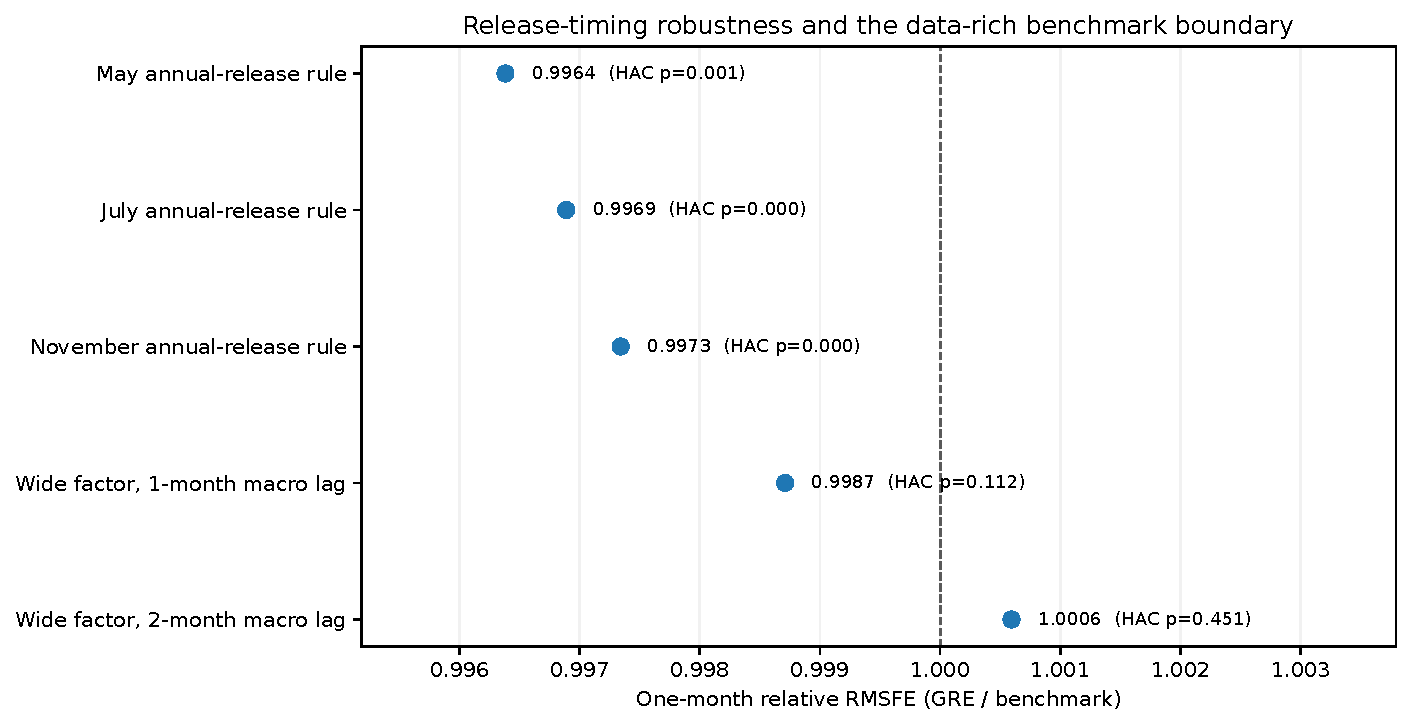
\includegraphics[width=0.90\textwidth]{Figure_Release_Benchmark_Boundary.pdf}
\caption{Release-timing robustness and the data-rich benchmark boundary at
the one-month horizon.}
\label{fig:release_benchmark}
\begin{singlespace}\footnotesize\textit{Notes:} Points report relative RMSFE
for GRE versus the corresponding benchmark. The first three rows vary the
assumed annual GDP release month under the parsimonious publication-lagged
benchmark. The final two rows augment the conventional information set with
six principal components extracted from 159 retained macroeconomic series.
Parenthetical values are target-month HAC Clark--West $p$-values.
\end{singlespace}
\end{figure}

The one-month RMSFE improvement under the parsimonious benchmark is about 0.36
percent and the MAE improvement about 1.03 percent. These are modest effects.
They would not justify a costly news-processing infrastructure if point
forecasting were the only objective. Their operational relevance is more
plausible for institutions that already maintain news pipelines for
surveillance and can use GRE as a challenger variable between low-frequency
statistical releases.

At twelve months, enforcing target-information timing changes the sign of
the GRE comparison. The remaining short-horizon result survives
release-calendar changes and deduplication but weakens against a wide factor
benchmark, and the revision regression does not identify a clear mechanism.
The robustness exercises therefore separate the information-set reversal from
the smaller, benchmark-sensitive short-horizon GRE result.

\FloatBarrier
\section{Discussion and conclusion}

\subsection{What the evidence establishes}

A forecasting exercise that treats a final-vintage disaggregated path as
both an ex post outcome and historically available lagged information does not
reproduce the information set the forecaster faced. The admissibility condition
states the requirement in general; Proposition~1 quantifies the Denton case,
where off-diagonal annual-benchmark influence decays at rate
$|\mu| = 0.2647$ per year and alternates in sign. The Monte Carlo designs show
that the direction of the distortion depends on the DGP: retrospective
information can suppress a short-horizon signal or, under a persistent-state
calibration, produce an apparent long-horizon gain that disappears under
publication timing. The African application shows the same information-set
correction reversing the original 12-month conclusion.

In the African application, the retrospective 12-month GRE ratio of 0.9961
becomes 1.0048 under publication timing. A channel decomposition attributes
most of the change to correcting forecast-origin GDP lags, and the reversal
survives removing all 2020--2021 forecast targets (0.9976 retrospective,
1.0133 publication-lagged). The one-month result is small, heterogeneous, and
benchmark-dependent, though it strengthens to 0.9926 in 2022--2025. It
survives alternative release conventions and deduplication, but the full-sample
bootstrap interval includes zero and the wide factor benchmark absorbs most of
the incremental evidence. The one-month results are consistent with some short-horizon information when
the annual information set is sparse, but the magnitude is small and depends
on the benchmark.

When the target-construction operator uses future low-frequency benchmarks,
historical regressors should instead be built with origin-specific one-sided
reconstruction, actual vintage data, or explicit publication-lag rules.
Reporting retrospective and feasible-information results separately makes the
effect of the information-set correction visible.

\subsection{Limitations and future validation}

Our publication-lagged reconstruction uses final-vintage annual GDP data, not
historical real-time vintages. Annual observations treated as available at a
given origin may therefore incorporate revisions made after their initial
release. The May, July, and November release conventions are transparent
timing rules, not exact country-specific historical release calendars.

This limitation is separate from the disaggregation-weight leakage in
Section~2.3. That problem arises when annual benchmarks that had not yet been
released enter monthly values dated before the forecast origin; the
origin-specific reconstruction removes it. What remains is vintage uncertainty
in the annual observations treated as already available. The effect on
forecast comparisons is ambiguous in sign. Final-vintage observations may be
smoother and better measured, strengthening the benchmark and reducing GRE's
incremental contribution. Alternatively, subsequent revisions may embed information the forecaster did
not have, altering benchmark dynamics and loss comparisons. The
exercise is therefore a publication-lagged final-vintage evaluation, not a
fully real-time experiment. Replication with archived country-specific GDP
vintages and historical release calendars would be the natural extension,
leaving the disaggregation-weight result in Section~2.3 unchanged.

The news measure has its own limits. Deduplication shows that repeated
identical stories do not drive the short-horizon result, but we do not
re-estimate lexicons, severity rules, or emphasis weights, and the human-coding
workbook is a validation protocol, not a completed label set. Arabic-only
content may be under-detected by the English, French, and Portuguese
dictionaries. These limits, together with the small and heterogeneous GRE
gains and their attenuation under the 159-series factor benchmark, bound the
empirical claim. They do not affect the target-information result.

\paragraph{Funding} This research did not receive any specific grant from
funding agencies in the public, commercial, or not-for-profit sectors.

\begingroup
\small
\setlength{\bibsep}{0pt plus 0.2ex}
\begin{thebibliography}{99}

\bibitem[Croushore and Stark(2001)]{croushorestark2001}
Croushore, D., \& Stark, T. (2001). A real-time data set for macroeconomists.
\emph{Journal of Econometrics}, 105, 111--130.
https://doi.org/10.1016/S0304-4076(01)00072-0.

\bibitem[Croushore(2006)]{croushore2006}
Croushore, D. (2006). Forecasting with real-time macroeconomic data. In
G. Elliott, C. W. J. Granger, \& A. Timmermann (Eds.), \emph{Handbook of
Economic Forecasting} (Vol. 1, pp. 961--982). Elsevier.
https://doi.org/10.1016/S1574-0706(05)01017-7.

\bibitem[Ad{\"a}mmer et al.(2025)]{adaemmer2025}
Ad{\"a}mmer, P., Pr{\"u}ser, J., \& Sch{\"u}ssler, R. A. (2025). Forecasting
macroeconomic tail risk in real time: Do textual data add value?
\emph{International Journal of Forecasting}, 41, 307--320.
https://doi.org/10.1016/j.ijforecast.2024.05.007.

\bibitem[Ahir et al.(2022)]{ahir2022}
Ahir, H., Bloom, N., \& Furceri, D. (2022). The World Uncertainty Index.
NBER Working Paper 29763. https://doi.org/10.3386/w29763.

\bibitem[Ardia and Bluteau(2026)]{ardia2026}
Ardia, D., \& Bluteau, K. (2026). Optimal text-based time-series indices.
\emph{International Journal of Forecasting}, 42, 44--60.
https://doi.org/10.1016/j.ijforecast.2025.07.003.

\bibitem[Abeyie(2026)]{abeyie2026}
Abeyie, G. A. (2026). Beyond news headlines and TF-IDF: Enhancing text-based
forecasting models with validated collocations and improved attention.
\emph{International Journal of Forecasting}, 42, 752--773.
https://doi.org/10.1016/j.ijforecast.2025.09.002.

\bibitem[Bae(2024)]{bae2024}
Bae, J. (2024). Factor-augmented forecasting in big data.
\emph{International Journal of Forecasting}, 40, 1660--1688.
https://doi.org/10.1016/j.ijforecast.2024.02.004.

\bibitem[Denton(1971)]{denton1971}
Denton, F. T. (1971). Adjustment of monthly or quarterly series to annual
totals: An approach based on quadratic minimization. \emph{Journal of the
American Statistical Association}, 66, 99--102.
https://doi.org/10.1080/01621459.1971.10482227.

\bibitem[Eilers(2003)]{eilers2003}
Eilers, P. H. C. (2003). A perfect smoother. \emph{Analytical Chemistry}, 75,
3631--3636. https://doi.org/10.1021/ac034173t.

\bibitem[International Monetary Fund(2017)]{imfqna2017}
International Monetary Fund. (2017). \emph{Quarterly National Accounts
Manual: 2017 Edition}. Washington, DC: International Monetary Fund.

\bibitem[Baker et al.(2016)]{baker2016}
Baker, S. R., Bloom, N., \& Davis, S. J. (2016). Measuring economic policy
uncertainty. \emph{The Quarterly Journal of Economics}, 131, 1593--1636.
https://doi.org/10.1093/qje/qjw024.

\bibitem[Ba{\'n}bura et al.(2013)]{banbura2013}
Ba{\'n}bura, M., Giannone, D., Modugno, M., \& Reichlin, L. (2013).
Now-casting and the real-time data flow. In G. Elliott \& A. Timmermann
(Eds.), \emph{Handbook of Economic Forecasting} (Vol. 2A, pp. 195--237).
Elsevier. https://doi.org/10.1016/B978-0-444-53683-9.00004-9.

\bibitem[Bok et al.(2018)]{bok2018}
Bok, B., Caratelli, D., Giannone, D., Sbordone, A. M., \& Tambalotti, A.
(2018). Macroeconomic nowcasting and forecasting with big data. \emph{Annual
Review of Economics}, 10, 615--643.
https://doi.org/10.1146/annurev-economics-080217-053214.

\bibitem[Caldara and Iacoviello(2022)]{caldara2022}
Caldara, D., \& Iacoviello, M. (2022). Measuring geopolitical risk.
\emph{American Economic Review}, 112, 1194--1225.
https://doi.org/10.1257/aer.20191823.

\bibitem[Clark and West(2007)]{clarkwest2007}
Clark, T. E., \& West, K. D. (2007). Approximately normal tests for equal
predictive accuracy in nested models. \emph{Journal of Econometrics}, 138,
291--311. https://doi.org/10.1016/j.jeconom.2006.05.023.

\bibitem[Gentzkow et al.(2019)]{gentzkow2019}
Gentzkow, M., Kelly, B., \& Taddy, M. (2019). Text as data. \emph{Journal of
Economic Literature}, 57, 535--574.
https://doi.org/10.1257/jel.20181020.

\bibitem[Giannone et al.(2008)]{giannone2008}
Giannone, D., Reichlin, L., \& Small, D. (2008). Nowcasting: The real-time
informational content of macroeconomic data. \emph{Journal of Monetary
Economics}, 55, 665--676.
https://doi.org/10.1016/j.jmoneco.2008.05.010.

\bibitem[Qu et al.(2024)]{qu2024}
Qu, R., Timmermann, A., \& Zhu, Y. (2024). Comparing forecasting performance
with panel data. \emph{International Journal of Forecasting}, 40, 918--941.
https://doi.org/10.1016/j.ijforecast.2023.08.001.

\bibitem[Akgun et al.(2024)]{akgun2024}
Akgun, O., Pirotte, A., Urga, G., \& Yang, Z. (2024). Equal predictive ability
tests based on panel data with applications to OECD and IMF forecasts.
\emph{International Journal of Forecasting}, 40, 202--228.
https://doi.org/10.1016/j.ijforecast.2023.02.001.

\bibitem[Coroneo and Iacone(2025)]{coroneo2025}
Coroneo, L., \& Iacone, F. (2025). Testing for equal predictive accuracy with
strong dependence. \emph{International Journal of Forecasting}, 41,
1073--1092. https://doi.org/10.1016/j.ijforecast.2024.11.003.

\bibitem[Seo(2025)]{seo2025}
Seo, B. (2025). Econometric forecasting using ubiquitous news text:
Text-enhanced factor model. \emph{International Journal of Forecasting}, 41,
1055--1072. https://doi.org/10.1016/j.ijforecast.2024.11.001.

\bibitem[Stock and Watson(2002)]{stockwatson2002}
Stock, J. H., \& Watson, M. W. (2002). Macroeconomic forecasting using
diffusion indexes. \emph{Journal of Business \& Economic Statistics}, 20,
147--162. https://doi.org/10.1198/073500102317351921.

\bibitem[Stock and Watson(2004)]{stockwatson2004}
Stock, J. H., \& Watson, M. W. (2004). Combination forecasts of output growth
in a seven-country data set. \emph{Journal of Forecasting}, 23, 405--430.
https://doi.org/10.1002/for.928.

\bibitem[Timmermann(2006)]{timmermann2006}
Timmermann, A. (2006). Forecast combinations. In G. Elliott,
C. W. J. Granger, \& A. Timmermann (Eds.), \emph{Handbook of Economic
Forecasting} (Vol. 1, pp. 135--196). Elsevier.
https://doi.org/10.1016/S1574-0706(05)01004-9.

\bibitem[Zheng et al.(2024)]{zheng2024}
Zheng, T., Fan, X., Jin, W., \& Fang, K. (2024). Words or numbers?
Macroeconomic nowcasting with textual and macroeconomic data.
\emph{International Journal of Forecasting}, 40, 746--761.
https://doi.org/10.1016/j.ijforecast.2023.05.006.

\end{thebibliography}
\endgroup

\clearpage
\appendix
\makeatletter
\@addtoreset{table}{section}
\@addtoreset{figure}{section}
\@addtoreset{equation}{section}
\makeatother
\setcounter{table}{0}
\setcounter{figure}{0}
\setcounter{equation}{0}
\section{News-source registry and web collection}
The source registry contains 851 distinct newspaper and digital-news outlets covering all 54 African economies. Each registry record contains an outlet name, country, language label, and website. The median country has 13 registered sources, with a range from 2 to 66. The source universe is multilingual: English and French are the largest groups, with dedicated Arabic- and Portuguese-language outlets and additional national, regional, and multilingual sources. Registered sources need not be available in every month, so source counts are treated as an upper-level coverage frame rather than a balanced monthly panel.

Collection is implemented as a recurring country--newspaper--month web-scraping process. Raw article files contain titles and article text. Retrieval is monitored at the source-month level. A source returning at least 20 percent fewer articles than in the preceding month enters scheduled retry passes. Only the strongest successful scrape for a newspaper-month is retained; multiple attempts are never concatenated. Cross-source duplicate screening is applied during collection, and completed monthly data are promoted to the historical archive only after the collection and processing stages complete successfully. These rules are designed to separate genuine changes in news volume from temporary website failures, incomplete retrieval, and repeated requests.

The frozen analytical archive contains 21,303,573 retained article records from January 2015 through December 2025. A total of 5,896,776 records satisfy the economic-relevance rule. The archive contains 7,127 country-month observations; 6,488 have at least 100 retained articles and the median country-month contains 1,039 records. Missing or unreadable source-months remain distinguishable from observed months with no qualifying risk content.

The unit of measurement is an article record, not an inferred independent news event. Cross-source screening cannot eliminate every syndicated, translated, or edited copy. A reconstructed exact-text audit removes 497,091 repeated records (2.33 percent), including 186,379 exact copies appearing across outlets. The forecast signal uses the frozen production vintage; the duplicate audit is reported as a corpus-quality diagnostic rather than substituted ex post for the measured signal.

\begin{table}[htbp]
\centering
\caption{News-source registry summary}
\begin{tabular}{lr}
\toprule
Registered newspaper and digital-news sources & 851\\
African economies covered & 54\\
Median registered sources per country & 13\\
Minimum registered sources in a country & 2\\
Maximum registered sources in a country & 66\\
Retained article records, 2015--2025 & 21,303,573\\
Economically relevant records & 5,896,776\\
Country-month observations & 7,127\\
Country-months with at least 100 articles & 6,488\\
\bottomrule
\end{tabular}
\end{table}

Figure~\ref{fig:coverage} reports the number of countries with at least 100 retained articles by month.
\begin{figure}[htbp]
\centering
\includegraphics[width=0.82\textwidth]{Supplement_Figure_Coverage.pdf}
\caption{Monthly news-coverage diagnostic.}
\label{fig:coverage}
\end{figure}

A GRE archive-depth regression over the 6,488 country-months satisfying the 100-article criterion gives a log-article-volume coefficient of 0.103 with country fixed effects ($p=0.656$), and 0.100 with both country and month fixed effects ($p=0.713$). These diagnostics do not establish source representativeness but provide little evidence of a mechanical within-country relation between GRE and archive size.


\section{GDP-PPP data provenance and target-information audit}
The annual activity input is the exact series labelled ``GDP (PPP)-WEO'' in the author-supplied workbook \nolinkurl{GDP_Data_African_countries_AUTHOR_SUPPLIED_2026-09-13.xlsx}. The replication package freezes that workbook as supplied on 13 September 2026 and provides the cleaned country-year extract \nolinkurl{annual_gdp_ppp_weo_labeled_final_vintage_2015_2025.csv}. The workbook does not contain an IMF WEO publication-release identifier. The paper therefore treats the observations as final-vintage WEO-labelled data and does not claim that they reproduce the historical values available to forecasters at each origin.

The final-vintage monthly evaluation target is constructed by additive first-difference Denton. If $Y_c$ stacks annual benchmarks, $G_c^F$ stacks monthly values, $D$ is the first-difference operator, and $A$ maps months into annual sums, then
\[
\min_{G_c^F}(DG_c^F)'(DG_c^F)\quad\text{subject to}\quad AG_c^F=Y_c.
\]
The monthly values reaggregate exactly to the annual benchmarks. The realized target is $100[\log G^F_{ct}-\log G^F_{c,t-12}]$.

The critical information-timing distinction is that $G_c^F$ is \emph{not} supplied to the forecasting model as if it had been observed historically. For every forecast origin the script reconstructs a separate GDP history from annual benchmark years allowed by the release convention. Under the baseline May rule, annual year $y$ is not available until May of $y+1$. Denton is applied only through the most recent permitted annual year; months after that year and through the forecast origin are extrapolated at the log-monthly rate implied by the two most recent permitted annual totals. A target dated in year $y$ cannot enter the recursive training sample before May of $y+1$.

For example, at a January 2020 forecast origin the May rule permits annual benchmarks only through 2018, whereas a June 2020 origin permits 2019. The November sensitivity rule is more conservative: annual 2019 does not enter until November 2020. These rules prevent the 2020--2025 annual totals from mechanically shaping GDP lags before their assumed release dates.

The procedure still uses final-vintage values for annual years deemed released. It therefore does not remove revisions to previously released years. A genuine historical-vintage experiment would require archived country-level annual GDP vintages and release calendars for every economy. The revised manuscript states this limitation explicitly and uses the term ``publication-lagged final-vintage'' rather than ``real time'' or ``leakage-free.''


\section{Closed-form Denton weight characterization}
This section supplies the algebra behind Proposition 1 in the main paper. The result concerns the interior behavior of additive first-difference Denton with twelve months per annual block. It is a characterization of the linear disaggregation operator, not an additional empirical assumption.

Fix one year and write $p=e_{y-1}$ and $q=e_y$ for the monthly levels at the preceding and current year-end. Let $d_1,\ldots,d_{12}$ be the monthly first differences and $x_i=p+\sum_{j\leq i}d_j$ the within-year monthly levels. The two constraints are
\[
\sum_{i=1}^{12}d_i=q-p,
\qquad
12p+\sum_{i=1}^{12}(13-i)d_i=Y_y.
\]
With
\[
C=\begin{pmatrix}
1&\cdots&1\\
12&11&\cdots&1
\end{pmatrix},
\qquad
b=\begin{pmatrix}q-p\\Y_y-12p\end{pmatrix},
\]
the minimum-norm solution is $d=C'(CC')^{-1}b$. Here
\[
CC'=\begin{pmatrix}12&78\\78&650\end{pmatrix},
\qquad
(CC')^{-1}=\begin{pmatrix}25/66&-1/22\\-1/22&1/143\end{pmatrix}.
\]
The minimized within-year roughness is therefore
\begin{equation}
R(p,q,Y)
=\frac{Y^2}{143}-\frac{Yp}{13}-\frac{Yq}{11}
 +\frac{23p^2}{78}+\frac{pq}{3}+\frac{25q^2}{66}.
\label{eq:s_R}
\end{equation}

The full Denton problem reduces to minimizing $\sum_y R(e_{y-1},e_y,Y_y)$ over the year-end sequence. Differentiating the two adjacent block contributions with respect to an interior $e_y$ gives
\begin{equation}
\frac{1}{3}e_{y-1}+\frac{578}{429}e_y+\frac{1}{3}e_{y+1}
=\frac{Y_y}{11}+\frac{Y_{y+1}}{13}.
\label{eq:s_boundary_recursion}
\end{equation}
The associated homogeneous characteristic equation is
\[
\frac{1}{3}+\frac{578}{429}z+\frac{1}{3}z^2=0,
\]
with roots
\[
\mu=\frac{12\sqrt{438}-289}{143}\approx-0.2647454934,
\qquad
\mu^{-1}\approx-3.7772125485.
\]
Because the two off-diagonal coefficients in equation~\eqref{eq:s_boundary_recursion} are equal, the roots are reciprocal. The bounded doubly-infinite solution retains only $\mu$ in the tail. A benchmark $Y_s$ enters the right-hand side of equation~\eqref{eq:s_boundary_recursion} only at two adjacent annual boundary equations, so outside those directly forced blocks its effect on $e_y$ is proportional to $\mu^{|y-s|}$.

Back-substitution provides the exact within-year interpolation formula. For month $r\in\{1,\ldots,12\}$,
\begin{equation}
x_{y,r}
= a_r e_{y-1}+b_r e_y+c_rY_y,
\qquad
a_r=\frac{(r-12)(3r-13)}{156},\quad
b_r=\frac{r(3r-25)}{132},\quad
c_r=\frac{r(12-r)}{286}.
\label{eq:s_monthly_backsub}
\end{equation}
Hence the annual-benchmark weights inherited by any interior month also have geometric off-diagonal tails. In particular, for a month $t=(y_0,r)$ there are constants $C_r^+$ and $C_r^-$ such that
\[
H_{t,y_0+k}=C_r^+\mu^{k-1},\qquad
H_{t,y_0-k}=C_r^-\mu^{k-1},\qquad k\geq1.
\]
The constants differ by month because the first off-diagonal exposure is determined by equation~\eqref{eq:s_monthly_backsub}. This distinction matters: $|\mu|$ is the exact ratio between successive tail coefficients, not a universal ratio of the first future-year coefficient to the own-year coefficient.

\input{tables/S_Denton_Weight_Profile.tex}

The table shows that first-future-year exposure can be small or substantial depending on the month and can change sign within the year. Once that first off-diagonal term is fixed, however, the next annual coefficient is always $\mu$ times the preceding one in the interior solution. The negative root therefore generates alternating signs, while $|\mu|<1$ produces rapid attenuation.

As a finite-sample check, the replication package reconstructs the exact 132-month Denton map for the 2015--2025 sample and compares successive off-diagonal ratios with the interior root. For a central 2018 annual block, the first and second future-tail ratios differ from $\mu$ by approximately $1.1\times10^{-7}$ and $1.6\times10^{-6}$, respectively; deviations grow as the opposite sample boundary is approached. The files \nolinkurl{GDP_Construction/denton_weight_characterization/denton_interior_month_profile.csv}, \nolinkurl{denton_geometric_decay.csv}, and \nolinkurl{denton_finite_sample_crosscheck.csv}, together with \nolinkurl{verify_denton_weight_decay.py}, reproduce the calculations.

\section{Monte Carlo design and full simulation results}
The Monte Carlo exercise isolates target-information treatment from the institutional details of the African application. Each replication contains 54 economies from 2015 through 2025, annual GDP is temporally disaggregated with the same first-difference Denton operator used in the paper, and the benchmark conditions on three lags of twelve-month growth and country fixed effects. The retrospective design supplies the complete final-vintage Denton history; the publication-lagged design admits annual year $y$ only from May of $y+1$.

Three DGPs are reported. The \emph{current-state signal} is intentionally modest: the alternative variable measures the contemporaneous annual activity innovation with noise and contains no next-year innovation. It is calibrated to produce a small feasible short-horizon gain. The \emph{pure-noise placebo} replaces the signal with independent noise. The \emph{persistent-state stress} DGP raises annual persistence from 0.25 to 0.95 and increases the signal-to-noise ratio. It is chosen only to establish an existence result in which the retrospective design generates the same direction of 12-month reversal observed in the African data. It is not intended to match the full empirical horizon profile or identify the mechanism generating the empirical reversal.

\begin{table}[htbp]
\centering\scriptsize
\caption{Full Monte Carlo results across three DGPs}
\begin{tabular}{llrrr}
\toprule
DGP & Design & $h$ & Mean rel. RMSFE & Share $<1$\\
\midrule
Current-state & Retrospective & 1 & 1.0002 & 39.0\%\\
Current-state & Publication-lagged & 1 & 0.9969 & 97.7\%\\
Current-state & Retrospective & 3 & 1.0002 & 36.6\%\\
Current-state & Publication-lagged & 3 & 0.9973 & 96.5\%\\
Current-state & Retrospective & 6 & 1.0002 & 39.2\%\\
Current-state & Publication-lagged & 6 & 0.9987 & 84.6\%\\
Current-state & Retrospective & 12 & 1.0001 & 47.5\%\\
Current-state & Publication-lagged & 12 & 1.0025 & 47.6\%\\
\midrule
Persistent-state stress & Retrospective & 1 & 1.0042 & 12.3\%\\
Persistent-state stress & Publication-lagged & 1 & 0.8715 & 100.0\%\\
Persistent-state stress & Retrospective & 3 & 1.0024 & 10.1\%\\
Persistent-state stress & Publication-lagged & 3 & 0.8793 & 100.0\%\\
Persistent-state stress & Retrospective & 6 & 0.9990 & 73.2\%\\
Persistent-state stress & Publication-lagged & 6 & 0.9149 & 100.0\%\\
Persistent-state stress & Retrospective & 12 & 0.9962 & 90.2\%\\
Persistent-state stress & Publication-lagged & 12 & 1.0122 & 35.1\%\\
\midrule
Pure-noise placebo & Retrospective & 1 & 1.0002 & 34.5\%\\
Pure-noise placebo & Publication-lagged & 1 & 1.0001 & 42.0\%\\
Pure-noise placebo & Retrospective & 12 & 1.0001 & 43.1\%\\
Pure-noise placebo & Publication-lagged & 12 & 1.0015 & 46.5\%\\
\bottomrule
\end{tabular}
\end{table}

The two signal DGPs deliberately demonstrate different distortions. In the modest current-state DGP, retrospective final-vintage history largely suppresses feasible short-horizon value and does not create a 12-month gain. In the persistent-state stress DGP, the 12-month retrospective ratio falls to 0.9962 while the publication-lagged ratio rises to 1.0122, reproducing the direction of the empirical reversal. The stress design's much larger short-horizon effects show why it should not be read as an empirical calibration. The pair of simulations supports the general admissibility result: the sign and horizon location of the distortion depend on persistence, signal strength, and how the constructed target enters the benchmark. The placebo shows that the procedure does not mechanically turn unrelated noise into a useful predictor.

\section{Publication-lagged horizon profile}
The baseline results use the May release convention, 2015--2018 frozen text scaling, and January 2020--December 2025 target dates.
\begin{table}[htbp]
\centering\scriptsize
\caption{Full horizon profile under the May release convention}
\begin{tabular}{rrrrrrrr}
\toprule
$h$ & Benchmark RMSFE & GRE RMSFE & Rel. RMSFE & Rel. MAE & HAC CW $p$ & Two-way $p$ & Target months\\
\midrule
1 & 8.375 & 8.344 & 0.9964 & 0.9897 & 0.0006 & 0.053 & 72\\
3 & 8.493 & 8.473 & 0.9977 & 0.9928 & 0.041 & 0.084 & 72\\
6 & 8.588 & 8.620 & 1.0037 & 1.0028 & 0.878 & 0.869 & 72\\
12 & 19.264 & 19.357 & 1.0048 & 1.0122 & 0.905 & 0.872 & 72\\
\bottomrule
\end{tabular}
\end{table}

Holm correction across the four target-month HAC values gives adjusted $p=0.0023$ at one month and 0.122 at three months. The corresponding two-way adjusted values are 0.211 and 0.253. The result is therefore strongest under the target-month aggregation that directly preserves the contemporaneous country cross-section; the two-way calculation is a complementary, more conservative diagnostic in the baseline May specification.

\end{document}